\documentclass[11pt,letterpaper]{article}
% \documentclass[man]{apa7}

\usepackage{showlabels}
\usepackage{fullpage}
\usepackage{pslatex}
\usepackage[english]{babel}
\usepackage[utf8]{inputenc}
\usepackage{amsmath}
\usepackage{bm}
\usepackage{xcolor}
\usepackage{url}
\usepackage{rotating}
%\usepackage{natbib}
\usepackage{amssymb}
\usepackage{lingmacros}


%\usepackage{linguex}
%\usepackage{lingmacros}
%\usepackage{CJKutf8}
%\newcommand{\korean}[1]{\begin{CJK}{UTF8}{mj}#1\end{CJK}}

\usepackage{tikz}


\usepackage{colortbl}

%\usepackage{xeCJK}
%\usepackage{natbib}

\bibliographystyle{unsrtnat}

%\usepackage{latexsym}
\usepackage[english]{babel}
\usepackage[utf8]{inputenc}
%\usepackage{bm}
\usepackage{graphicx}
%\usepackage{tikz}
\usepackage{xcolor}
\usepackage{url}
%\usepackage[colorinlistoftodos]{todonotes}
\usepackage{rotating}
\usepackage{multirow}
\usepackage{hyperref}
\usepackage{tikz-dependency}
\usepackage{changepage}
\usepackage{longtable}

\usepackage{csquotes}
\usepackage[bibencoding=utf8, style=apa,sortcites=true,sorting=nyt,backend=biber]{biblatex}
%\usepackage[backend=biber, bibencoding=utf8, style=authoryear, citestyle=authoryear]{biblatex} % https://tex.stackexchange.com/questions/402714/biblatex-not-working-with-biber-2-8-error-reading-bib-file-in-ascii-format
\DeclareLanguageMapping{american}{american-apa}
\addbibresource{literature.bib}



\title{Morpheme Ordering across Languages reflects Optimization for Processing Efficiency}


%\leftheader{Anonymous}




\newcommand{\citep}{\parencite}
\newcommand{\citet}{\Textcite}



\newcommand{\R}[0]{\mathbb{R}}
\newcommand{\Prob}[0]{\mathbb{P}}
\newcommand{\Ff}[0]{\mathcal{F}}

\usepackage{multirow}

\newcommand{\soft}[1]{}
\newcommand{\nopreview}[1]{}
\newcommand\comment[1]{{\color{red}#1}}
\newcommand\michael[1]{{\color{red}(#1)}}
\newcommand\mhahn[1]{{\color{red}(#1)}}
\newcommand\becky[1]{{\color{blue}(#1)}}
\definecolor{Pink}{RGB}{255,50,170}
\newcommand{\jd}[1]{\textcolor{Pink}{[jd: #1]}}  
\newcommand{\key}[1]{\textbf{#1}}

\DeclareMathOperator*{\argmax}{arg\,max}
\DeclareMathOperator*{\argmin}{arg\,min}
\DeclareMathOperator{\E}{\mathop{\mathbb{E}}}



%\usepackage{lingmacros}
%\usepackage{linguex}


\usepackage{amsthm}

\newcommand{\thetad}[0]{{\theta_d}}
\newcommand{\thetal}[0]{{\theta_{LM}}}

\newcounter{theorem}
\newcounter{def}
\newtheorem{proposition}[theorem]{Proposition}
\newtheorem{thm}[theorem]{Theorem}
\newtheorem{definition}[def]{Definition}
\newtheorem{corollary}[theorem]{Corollary}
\newtheorem{question}[theorem]{Question}
\newtheorem{example}[theorem]{Example}
\newtheorem{lemma}[theorem]{Lemma}

%\abstract{
%}

%\keywords{Language universals, sentence processing, information theory}

%\authornote{
%   \addORCIDlink{Michael Hahn}{0000-0003-4828-4834}
%
%  Correspondence concerning this article should be addressed to Michael Hahn, Department of Linguistics, Stanford University Stanford, CA 94305-2150.  E-mail: mhahn2@stanford.edu
%  
%All code and data is freely available at \url{https://github.com/beckymathew/morpheme-ordering}.
%  }

\renewcommand{\thefigure}{S\arabic{figure}}
\renewcommand{\thetable}{S\arabic{table}}
\renewcommand{\thesection}{S\arabic{section}}

\newcommand{\utterance}{\mathcal{U}}
\newcommand{\tree}{\mathcal{T}}




\usepackage{longtable}



%\frenchspacing
%\def\baselinestretch{0.975}

%\emnlpfinalcopy
%\def\emnlppaperid{496}


\begin{document}


\maketitle

\begin{abstract}
    The order of morphemes in a word displays well-documented regularities across languages.
Previous work has explained these in terms of notions such as semantic scope and relevance. 
A recent theory argues that word and morpheme order in language optimizes a tradeoff between memory and surprisal, and provided initial evidence from two languages that morpheme order can partly be explained by optimization for this tradeoff.
In this work, we test this idea more extensively using data from four additional agglutinative languages with significant amounts of morphology, in both verb and noun inflection.
We find that the memory-surprisal tradeoff predicts order in most cases with high accuracy, and accounts for crosslinguistic regularities in noun and verb inflection.
Our work adds to a growing body of work suggesting that many ordering properties of language arise from a pressure for efficient language processing.
\end{abstract}


%\begin{abstract}
%\end{abstract}

\section{Introduction}

Human language encodes thoughts into linear strings of words, and ultimately sounds.
Across languages, words are composed of morphemes, commonly defined as the smallest meaning-bearing units of language~\citep{courtenay1895attempt,bloomfield1926a,katamba2006morphology}.
%In many cases, words can be segmented into a sequence of morphemes, as in
For instance, the English word ``runners'' can be decomposed into three morphemes: the root \textit{run-} indicating an action, the suffix \textit{-er-} indicating someone performing an action, and plural \textit{-s} indicating a group of several referents.
The order of morphemes within a word follows well-documented cross-linguistic tendencies \citep{greenberg-universals-1963, bybee-morphology-1985, baker1985the}. For instance, derivational morphemes (e.g., English \textit{-er} deriving nouns from verbs) are ordered closer to the root than inflectional morphemes (e.g., English plural \textit{-s}).
%
%Another well-documented universal applying to languages with richer morphology is Greenbergs' Universal 39:
%Plural markers tend to be closer to noun stems than case markers \citep[112]{greenberg1963universals}. %(see Section~\ref{sec:univ-nouns} below).
%
In morphologically rich languages, nouns and verbs often have a string of two or more affix morphemes attached to a root, and the typological literature has documented universal tendencies, such as a preference for plural markers to be closer to noun stems than case markers \citep{,greenberg1963universals,bybee-morphology-1985}. 

Explaining these linguistic universals has been an important subject of study \citep{bybee-morphology-1985, spencer2006linguistic, manova2010modeling, bauer2010an, rice2011principles,hay2004what}.
Explanations of morpheme ordering have been stated in terms of correspondences between morpheme order \jd{be consistent in use of "order" vs "ordering"} and morpheme meanings \citep{bybee-morphology-1985,rice2000morpheme,saldana2021cross}, parallelism between morphology and syntax \citep{givon1971historical,venneman1973explanation,baker1985the}, and human morphological processing and usage frequencies \citep{hay2002speech, plag2002the, inkelas2016affix}.
%\jd{can a generalization be drawn about the high-level ways in which these accounts differ?}
Explanations of the first kind state that morphemes are ordered based on differences in semantic scope \citep{rice2000morpheme} or relevance \citep{bybee-morphology-1985}, such that morphemes that are more semantically similar to the root occur closer to it.
Explanations of the second kind propose that the order of morpheme mirrors the order of independent words with corresponding meanings, due to either language history or synchronic constraints on language.
Explanations of the third kind argue that affixes are closer to the root when they are more likely to be processed together with it in dual-route models of lexical access \citep{baayen-frequency-1993}.

A recent theory proposes a cognitive explanation for word and morpheme order in language, arguing that ordering universals in language optimize processing effort under memory limitations \citep{Hahn2020modeling}.
\citet{Hahn2020modeling} introduce the notion of a \emph{memory-surprisal tradeoff}: The more memory resources a comprehender invests in representing the context preceding the currently observed word, the lower the achievable surprisal that the comprehender must incur on that word. Conversely, the less memory is invested, the higher the surprisal.
\citet{Hahn2020modeling} argue that order of words and morphemes in language optimizes this tradeoff.
They show that optimizing the memory-surprisal tradeoff amounts to placing elements close together that strongly predict each other, as measured by mutual information.
%They also suggest that mutual information formalizes previous notions of strength of semantic association between morphemes \citep{bybee-morphology-1985}. %, such as \cite{bybee-morphology-1985}'s notion of \textit{relevance}.
\citet{Hahn2020modeling} argue that this property of the memory-surprisal tradeoff generalizes previous processing theories which suggest that orderings tend to place together elements that are syntactically related \citep{rijkhoff-word-1986, hawkins-performance-1994}, conceptually related \citep{givon1985iconicity}, semantically relevant to each other \citep{bybee-morphology-1985}, or processed together in lexical access \citep{hay2004what}.
While focused on explaining word order across 54 languages, \citet{Hahn2020modeling} also test whether two languages optimize the memory-surprisal tradeoff at the morphological level. In particular, they find that optimizing the memory-surprisal tradeoff partly reproduces the morpheme order of Japanese and Sesotho.


%that the memory-surprisal tradeoff is more efficient when elements that are highly predictive of each other are placed together more closely.
% \citep{Hahn2020modeling}
%\mhahn{TODO here say more about how the tradeoff differs from other processing theories.}
%relation to prior processing proposals:
%- surprisal
%- locality -- generalized to information locality


Here, we test this theory on a broader basis.
We consider data from four agglutinative languages -- i.e., languages with rich morphology where words tend to have multiple morphemes which are mostly realized separately (Korean, Turkish, Hungarian, and Finnish) -- in addition to the two language already considered by \citet{Hahn2020modeling} (Japanese and Sesotho).
These languages have very substantial verbal inflection, and three of these languages (Turkish, Hungarian, Finnish) also have substantial noun inflection. We test both whether the memory-surprisal tradeoff accounts for universals of verb affix order documented by \cite{bybee-morphology-1985}, but also extend the scope of the analysis to nouns, where we test whether the theory accounts for Greenberg's Universal 39 \citep{greenberg-universals-1963}. %\jd{this universal has not been introduced yet}

\jd{say something either here or in section 2 about the relationship between the languages under consideration -- eg, how many language families are represented}

The six languages under consideration represent five language families (Korean, Japonic, Uralic, Turkic, Niger-Congo).
Finnish and Hungarian both belong to the Uralic family, sharing a common ancestor about 5,000 years ago \citep{maurits2020best}.
The other languages in the sample are not genetically related according to their generally accepted classification.
%Importantly, the morphemes found in these languages as considered here are largely not cognate.
%Thus, the commonalities in languages found cannot be traced to inherited orderings of morphemes inherited from a common ancestor.


% interesting https://www.eva.mpg.de/fileadmin/content_files/staff/haspelmt/pdf/Agglutination.pdf

%Greenberg 1963:  "the expression of number almost always comes between the noun base and the expression of case" (Greenberg 1963:112)

%Scope, Syntax, History
%Another family of explanations holds that morpheme ordering is to be explained diachronically, and that morpheme order reflects the order of independent words in earlier stages of a language.
%- Relevance, Proximity Principle, Iconicity




%Bybee on explanation:
%- regarding the historical explanation (Givon 1971, Vennemann 1973):
%Morphology is not always fossilizes syntax (Bybee and Brewer 1980, Bybee 1985 p. 39--40)


\section{Morpheme Ordering and Ordering Universals}\label{sec:univ}


In this section, we introduce the phenomena we seek to explain: crosslinguistic tendencies in the order of affix morphemes in nouns (Section~\ref{sec:univ-nouns}) and verbs (Section~\ref{sec:univ-verbs}).
Languages apply affix morphemes to different classes of words, including both open word classes such as nouns, verbs, and adjectives, and closed word classes, in particular pronouns.
In this work, we focus on open word classes, as these have productive paradigms that apply to thousands of words in a language, including words that newly enter the language, whereas pronominal inflection is restricted to a small number of words, often with idiosyncratic and fossilized paradigms inherited from earlier stages of a language.
Among open word classes, inflection commonly applies to verbs, nouns, and adjectives.
When adjectives are inflected, they often pattern with either verbs -- when they are used as predicates -- or nouns -- when they are used as attributes or independent nouns.
We thus focus on nouns and verbs, treating adjectives together with one of the other classes depending on the language when appropriate (with verbs in Korean and Japanese; with nouns in Hungarian, Finnish, Turkish).

\subsection{Universals of Noun Affix Ordering}\label{sec:univ-nouns}
Nouns very commonly mark number and case morphologically.
%Number marking typically distinguishes singular and plural (person -- person-s).
%Case marking 
In some languages, possession is also marked on the noun.
Figure~\ref{fig:noun-inflection} shows fully inflected nouns in three languages from our sample, with endings for number, case, and possessor.
Number and case marking are the subject of a well-documented universal, namely \citet{greenberg1963universals}'s Universal 39:

\begin{adjustwidth}{6em}{6em}
\textsc{Greenberg's Universal 39}:
``the expression of number almost always comes between the noun base and the expression of case'' (Greenberg 1963:112).
\end{adjustwidth}
%It states that number affixes are closer to the stem than case affixes, if they appear on the same side.
This universal is supported by the example in Figure~\ref{fig:noun-inflection}.

%\ex.\ag. mi  rare mash yoo \\
%%Stem (3) (5) (8) \\
%see  \textsc{passive}  \textsc{politeness}  \textsc{future} \\
%`will be seen'
%\bg. mi taku nakat ta \\
%%Stem (6) (7) (8) \\
%see \textsc{desiderative} \textsc{negation} \textsc{past} \\
%`did not wish to see'


\begin{figure}
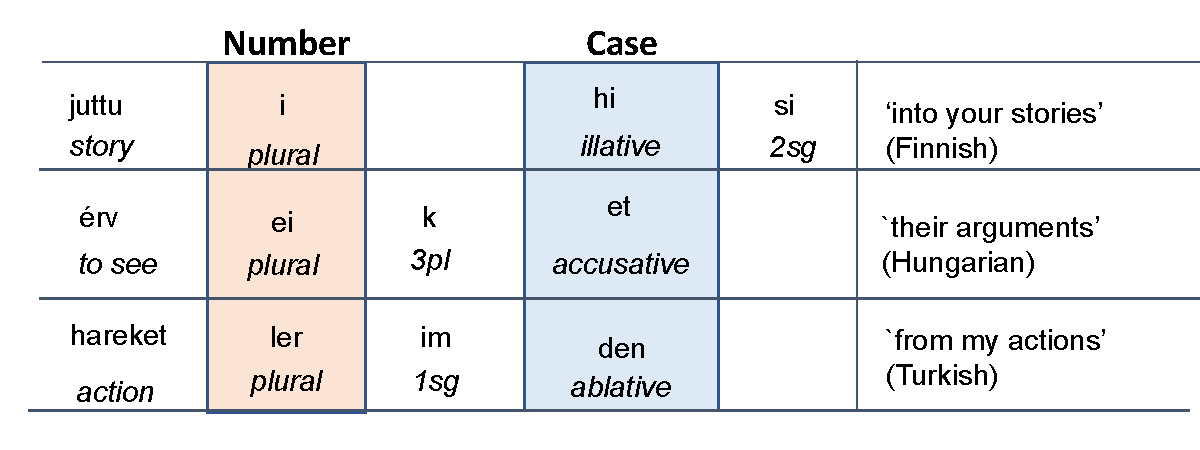
\includegraphics[width=0.8\textwidth]{figures/noun-morphemes.pdf}
%\begin{tabular}{lllllllll}
%\textit{juttu-i-hi-si} \\
%%Stem-Plural-Illative-2SgPoss \\
%`into your stories' (Finnish)
%\end{tabular}
%\begin{tabular}{lllllllll}
%	\textit{{\'e}rv-ei-k-et} \\
%Stem-Plural-3rdPlurPoss-Accusative \\
%`their arguments' (Hungarian)
%\end{tabular}
%\begin{tabular}{lllllllll}
%\textit{hareket-ler-im-den} \\
%Stem-Plural-1sgPoss-Ablative\\
%`from my actions' (Turkish) \\
%\end{tabular}


\caption{Noun inflection in the three languages in our sample. All three languages support Greenberg's Universal 39 by placing the case marker after the plural marker, but they differ in the placement of the possessive marker.\jd{why is the possessive marker glossed as a person marker?} \mhahn{TODO make this look nicer}}\label{fig:noun-inflection}
\end{figure}



 \begin{figure}
 a)
 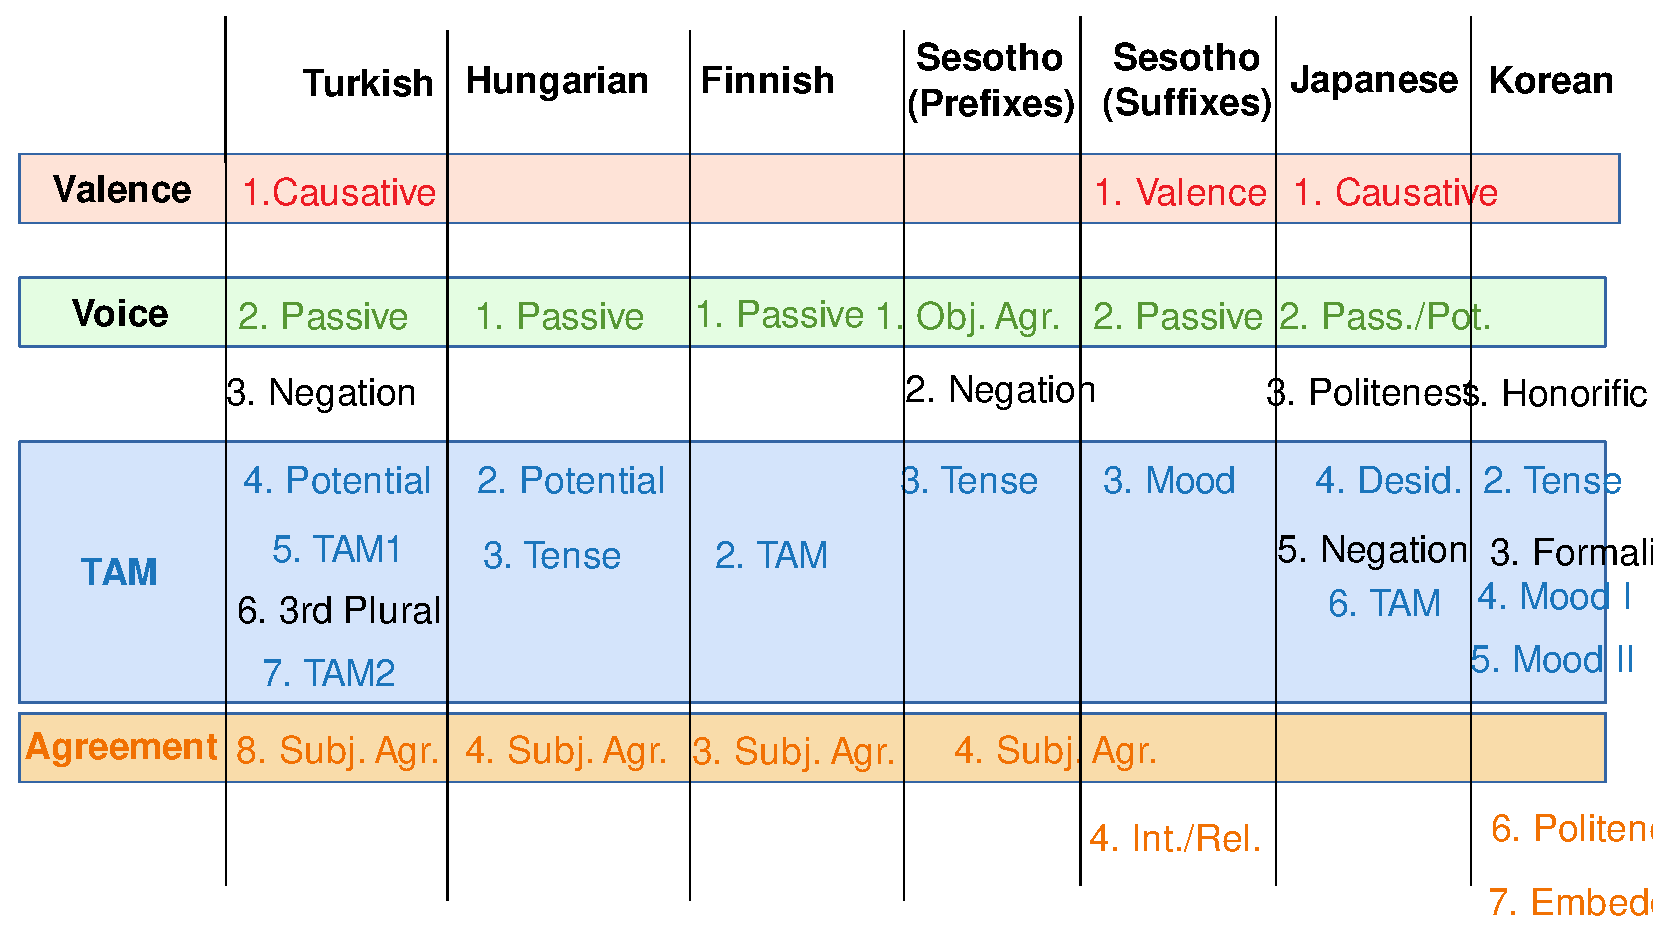
\includegraphics[width=0.7\textwidth]{figures/slots.pdf}
 
 b)     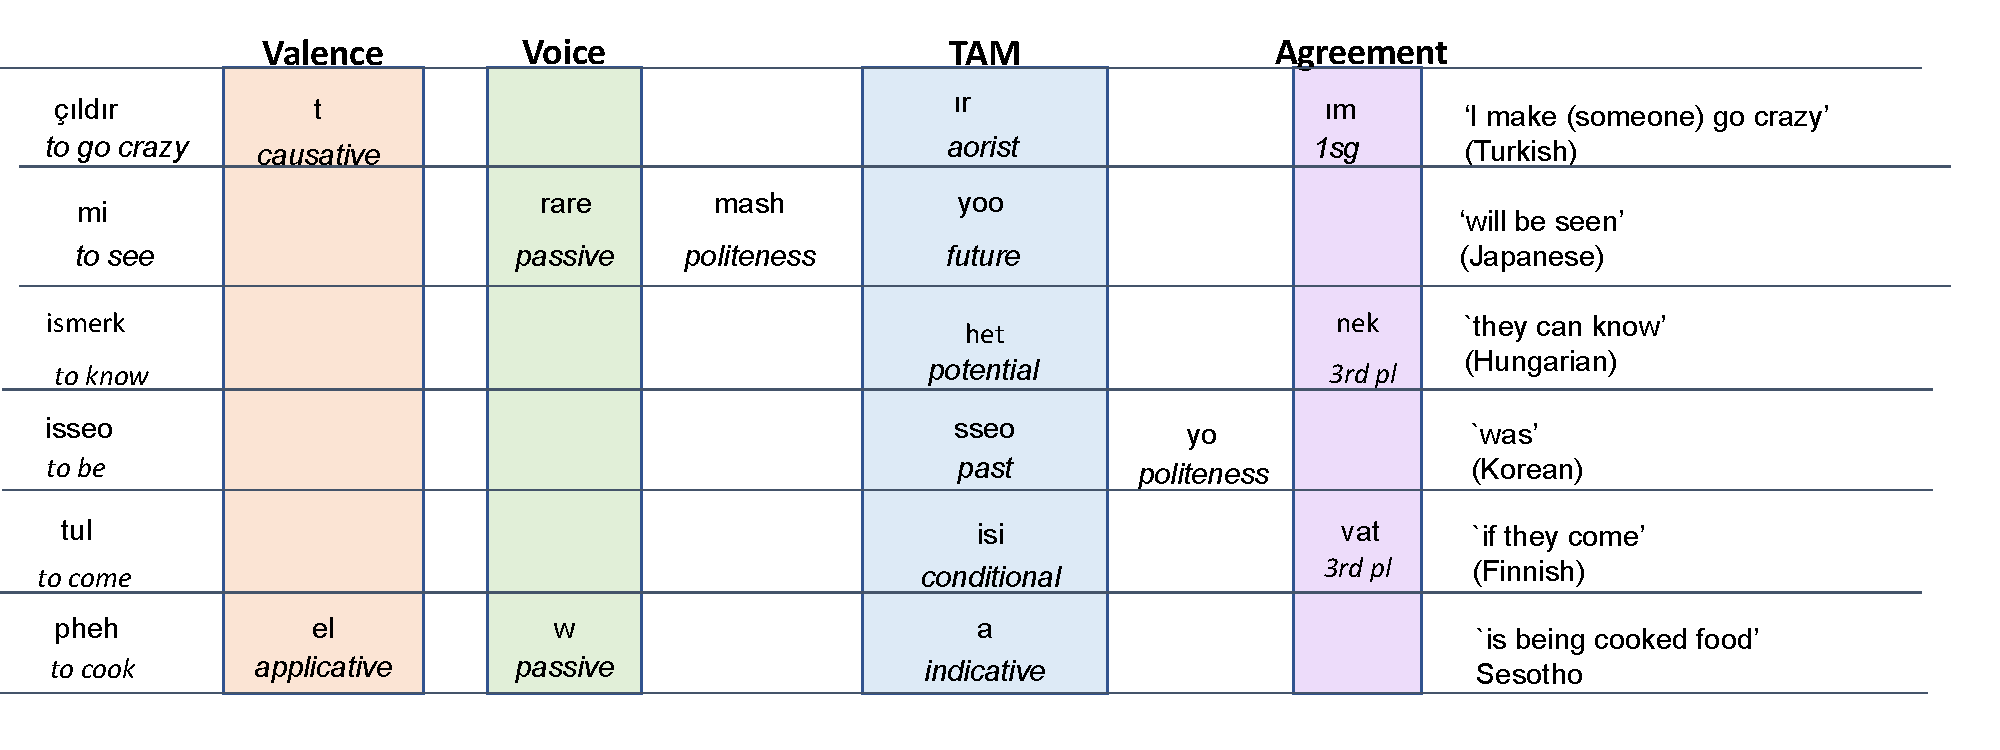
\includegraphics[width=\textwidth]{figures/verb-morphemes.pdf}
 
%     Valence:
%\begin{tabular}{lllll}
%	a) & {\c c}{\i}ld{\i}r-{\i}r-{\i}m \\
%& go.crazy-Causative-aorist-1sg \\
%& `I go crazy' (Turkish)\\
%b) & {\c c}{\i}ld{\i}r-t-{\i}r-{\i}m \\
%& go.crazy-Causative-aorist-1sg \\
%& `I make (someone) go crazy' (Turkish) \\
%\end{tabular}     
%Voice:
%\begin{tabular}{llllll}
%a) & mi-mash-yoo \\
%& see-politeness-future \\
%& `will see' (Japanese) \\
%b) & mi-rare-mash-yoo \\
%& see-passive-politeness-future \\
%&`will be seen' (Japanese)
%\end{tabular}%

%Mood:
%\begin{tabular}{llll}
%a) & ismer-nek \\
%& know-3pl.def \\
%& `they know' (Hungarian) \\
%b) & ismer-het-nek \\
%& know-potential-3pl.def \\
%& `they can know' (Hungarian)
%\end{tabular}
%Tense:
%\begin{tabular}{llllll}
%a) & isseo-yo \\ 
%& be-polite \\
%& `is/are' (informal polite, Korean) \\ 
%b) & isseo-sseo-yo \\
% & be-past-polite \\
% & `was/were' (informal, polite, Korean)
% \end{tabular}
% Agreement:
%\begin{tabular}{lllll}
%a) & a{\c c}ar-{\i}m \\
%b)& a{\c c}ar-s{\i}n \\
%c) & a{\c c}ar-{\i}z \\
%d) &a{\c c}ar-s{\i}n{\i}z \\
%& stem-person \\
%& `I/you (sgd)/we/you (pl) open'
%\end{tabular}

\mhahn{TODO make this rough draft look nice. also add derivational affixes as mentioned in the text}
\caption{(A) Verb affix slots in the six languages, grouped into four universal slots where applicable. Affixes are listed outwards from the root. (B) Examples of verb inflection from the six languages.}\label{tab:examples-verbs}
\end{figure}
 
 
% \begin{figure}
%     \centering
%     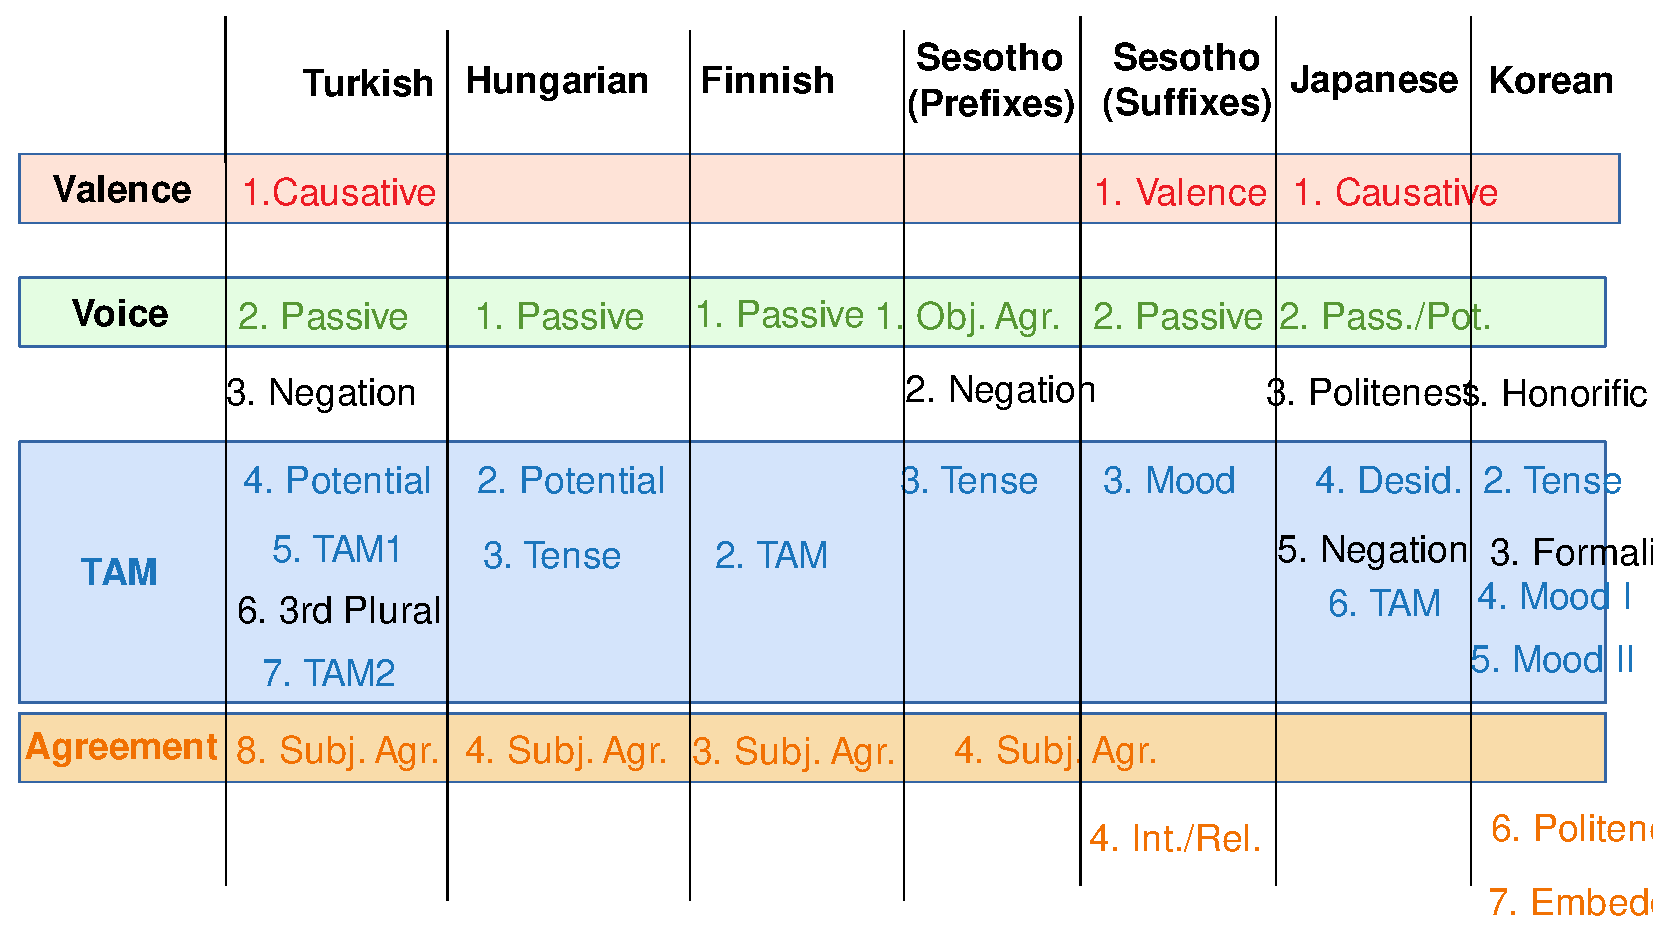
\includegraphics[width=\textwidth]{figures/slots.pdf}
%     \mhahn{todo make this rough draft look nice, and m,ake colors consistent with the other figure. also, add in derivational suffixes at the top}
     %\caption{Verb affix order across the six languages in our sample, matched with four universal categories (left). \mhahn{Question: We could think about removing his figure, while adding this color coding to Figures 8--9 to tighten the link to Figure 3. This figure here doesn't seem to add much beyond Figure 3, except for language-specific detail that isn't useful to the reader here. Its main advantage is that it prepares the reader to expect somewhat messy language-specific patterns later in Figure 8, but that could also be done by adding color coding there. What do you think?} }
%    \label{tab:examples-verbs}
% \end{figure}


\subsection{Universals of Verb Affix Ordering}\label{sec:univ-verbs}
Verbs commonly mark a larger number of inflection categories.
Figure~\ref{tab:examples-verbs} summarizes the affixes in the verbal morphologies of the six languages considered here (see SI Section S1 for details on how we arrived at these summaries).
Sesotho has both prefixes and suffixes; we treat these separately, as we only aim to explain the relative distance of affixes from the base, not which side of the verb they appear on.

Verb affixes are typically grouped into derivational and inflectional affixes.
Derivational affixes derive new verb stems (e.g., 'do' $\rightarrow$ undo), whereas inflectional affixes derive inflected verb forms from verb stems (e.g., `do' $\rightarrow$ `does').
Examples of derivational suffixes are Japanese -su- and Korean -ha-, which derive verbs from non-verbal stems \citep{hasegawa2014japanese, yeon2010korean}.
Another example is the reversive suffix in Sesotho (corresponding to `un-' in English `do' $\rightarrow$ `undo', \citep{doke1967textbook}.
Derivational affixes generally appear closer to the root than inflectional affixes \citep{greenberg-universals-1963}.

Languages can have several inflectional affixes stacked (Figure Figures~\ref{tab:examples-verbs}); their ordering shows universal tendencies \citep{bybee-morphology-1985}, which we summarize as follows:

\begin{adjustwidth}{6em}{6em}
\textsc{Verb Affix Ordering} \citep{bybee-morphology-1985}:
Verb affixes are ordered as follows, outward from the verb stem:

\begin{tabular}{llllllllllllllllllllllllll}
verb stem & valence & voice & TAM & subject agreement
\end{tabular}
\end{adjustwidth}

\textit{Valence} affixes (red in Figure~\ref{tab:examples-verbs}) change the number of arguments. A very common type of valence affix is a causative, which adds an argument indicating who causes an event or state to occur \citep{wals-111}.
\textit{Voice} (green in Figure~\ref{tab:examples-verbs}) describes the distinction between active and passive. % An example is the Japanese passive suffix -\textit{(r)are}- (Figure~\ref{tab:examples-verbs}).
\textit{Tense-Aspect-Mood (TAM)} (blue in Figure~\ref{tab:examples-verbs}) comprises three types of categories \citep[Tense-Aspect-Mood,][]{bybee1994the, wals-69}.
%An example of aspect marking is the English progressive \textit{to be} ...-\textit{ing}, which indicates that an action is currently ongoing \citep{huddleston-cambridge-2002}.
\textit{Tense} describes where an event is located in time (e.g. past or future).
\textit{Aspect} describes how an event unfolds over time \citep{comrie1976aspect,dahl1985tense,binnick1991time}.
%Examples of tense and aspect marking are shown in Figure~\ref{tab:examples-verbs}.
\textit{Mood} describes a relation between an event and the speaker, including an assessment of the event's reality \cite{palmer1986mood,portner2018mood}.
%In analytical languages such as English, mood distinctions are often indicated using verbs such as \textit{might} or adverbs such as \textit{possibly}.
A common mood category is the potential mood, which indicates possibility (Turkish, Hungarian).
%Figure~\ref{tab:examples-verbs} shows how it is marked morphologically with -het- in Hungarian \citep{rounds2001hungarian}.
Aspect and tense categories are often fused in morphology \citep{binnick2012the}, and mood marking is also often fused with those. %; for instance, the Japanese suffix -\textit{yoo} can mark future tense and the hortative mood (`let's ...', \citep{hasegawa2014japanese}).
Some languages have a single affix slot that accommodates a fused morpheme indicating TAM.
For instance, Finnish marks both tense (present and past) and mood (indicative, conditional, and potential) categories with a single morpheme in the slot labeled TAM.
Other languages have multiple slots, for instance, Turkish TAM markers are distributed across two slots (Figure~\ref{tab:examples-verbs}).

\textit{Subject agreement} (orange in Figure~\ref{tab:examples-verbs}) marks categories of the subject, most often its person and number, sometimes also other categories such as its gender \citep{corbett2003agreement}.
An example is English third-person \textit{-s}.
In our sample, Turkish, Hungarian, Finnish, and Sesotho have a subject agreement slot (Figure~\ref{tab:examples-verbs}); Turkish also has a special slot occupied only by the third-person plural marker \textit{-lar-} (indicated as 3rdPl in ~\ref{tab:examples-verbs}).


%Based on data from several dozens of languages, \citep{bybee-morphology-1985} proposes the following ordering of these common verb affixes:
%\begin{quote}
%\begin{tabular}{llllllllllllllllllllllllll}
%verb stem & valence & voice & aspect & tense& mood & subject agreement
%\end{tabular}
%\end{quote}

Figure~\ref{tab:examples-verbs} shows that the languages in our sample largely support the \textsc{Verb Affix Ordering} universal, with the exception of the order of the special third-plural suffix slot in Turkish, which intervenes between two TAM slots.
\citet{bybee-morphology-1985} also provides evidence for ordering preferences within aspect, tense, and mood; however, we do not distinguish between them as these are frequently fused in languages.


While these are particularly common types of affixes, there are further types, some of which occur in the six languages of our sample.
While agreement is most commonly established with the subject, \textit{agreement with the object} is found in Sesotho \citep{doke1967textbook} (in person and noun class) and in Hungarian \citep{rounds2001hungarian} (in definiteness); it is fused with subject agreement in the Hungarian and shares a slot with Valence in Sesotho (see SI Section S1.4).
\textit{Polarity} refers to the opposition between affirmative (e.g. `she arrived') and negative  (e.g., `she did not arrive') statements \citep{wals-112}.
\textit{Evidentiality} indicates on what evidence a speaker bases an assertion \citep{aikhenvald2003evidentiality}.
\textit{Formality}, \text{honorifics}, and \text{politeness} are categories that index social relations between the speaker, the addressee, and the topic of the conversation~\citep{hasegawa2014japanese, yeon2010korean}.
In our sample, these are prominent in Korean and Japanese.
The Japanese politeness marker -masu- and the Korean formality (-p) and politeness (-yo) suffixes index the social relation between the speaker and the addressee \citep{hasegawa2014japanese, yeon2010korean}; the Korean honorific suffix -si- indexes the social relation between the speaker and the topic of the conversation \citep{yeon2010korean}.
Furthermore, verb forms can have affixes indicating the syntactic position of the verb within a sentence, in particular, affixes marking infinitives or other nonfinite forms.
We use the term \textit{Syntactic} for this type of morpheme.

Having introduced the two universal generalizations about noun and verb affixes, we now review existing accounts of morpheme ordering (Section~\ref{sec:previous}). 

%\jd{add segue to next section}

%We focus on inflection, except in those cases where derivational affixes are clearly marked in available data.
%Inflectional suffixes are generally outside of derivational affixes

% somewhere explain the choice of languages
% - rich agglutinative.
% - must have data with suitable morphological analysis.
% - Among the languages, Hungarian and Finnish are genetically related (X millenia). There is also some evidence for genetic relations beyond these (Japanese, Korean, Turkish), but such relations would have to be quite ancient (x millenia).
% The morphemes found in these languages as considered here are generally not cognate.




\subsection{Previous Accounts of Morpheme Ordering}\label{sec:previous}

Here, we review previous explanatory accounts of morpheme ordering and motivate our study.
%In a review of research on morpheme ordering, \citet{manova2010modeling} % https://homepage.univie.ac.at/stela.manova/modeling%20affix%20order.pdf
%categorize approaches to morpheme ordering into three classes (similarly \citet{rice2000morpheme, rice2011principles}): orderings that are motivated by properties of syntax, semantics or phonology; orderings that are motivated by human language processing responding to statistical properties of language; and orderings that are arbitrarily stipulated.
%Our approach falls into the second class, explaining morpheme ordering based on minimization of human processing effort.
%In this section, we describe how our account relates to other accounts across these three \becky{four?} clusters, and show how the memory-surprisal tradeoff has tight connections with notions proposed across seemingly very different accounts.
Prominent accounts of morpheme ordering universals highlight the correspondence between morpheme ordering and semantics~\citep{bybee-morphology-1985,rice2000morpheme}.
\citet{bybee-morphology-1985} argues that ordering is determined by the semantic relevance of affixes to the root.
For example, she argues that morphemes that change a verb's argument structure, such as passives and causatives, have a particularly strong relation to the verb's semantics, as they fundamentally alter the nature of the event described, whereas tense or agreement markers are much less tightly linked to the verb's meaning.
Similarly, she argues that agreement markers are less relevant to the stem than TAM markers, since TAM interacts more closely with the verb's semantics; for instance, verbs denoting states or actions differ in the applicable aspect categories, but not in the applicable subject agreement features.
While the intuitive notion of relevance provides an appealing account of the \textsc{Verb Affix Ordering} generalization, applying it to novel languages as an explanatory and testable notion requires some kind of formal operationalization of relevance that also applies to other language-specific kinds of morphemes, such as negation and politeness.
%\jd{sounds accusatory. soften by highlighting which of the tendencies observed in section 2.2 and 2.3 this accounts for, which it doesn't, and then highlight that while the intuitive notion of relevance is appealing, it won't work as an explanatory notion when applied to novel languages unless operationalized formally in some way (or something like that)}

A second prominent semantic account holds that morphemes are ordered in the order in which their meanings combine, so that morphemes are closer to the root when their meanings have narrower scope \citep[e.g.,][]{rice2000morpheme, caballero2010scope,  narrog2010the, korotkova2010deriving}.
A good example for the scope-based explanation is the relative ordering of valence and voice.
Turkish has suffixes both for causative and passive.
When adding both suffixes simultaneously, the causative marker appears closer to the root.
The Turkish verb stem \textit{don} ``to freeze'' forms a causative \textit{don-dur} ``to freeze (something)''.
Futher applying a passive suffix results in \textit{don-dur-ul} ``to be frozen'' \citep[][Section 30.8.2]{schaaik2020turkish}.
The order of affixes corresponds to the order in which the meanings of these suffixes combine with the meaning of the root:
The causative affix adds an argument indicating who makes an object freeze, and the passive affix then removes that argument, yielding a verb describing something that is being frozen by someone.


While this account is successful at predicting the order of valence and voice (with the exception of anti-scope orderings in some languages, \citep{...}), it is less straightforwardly evaluated for other affixes because its predictions can depend on the specifics of how meaning is represented (see SI Section TODO for further discussion). %\jd{example?} \mhahn{TODO I'd prefer to place this discussion in an SI section, with some formal semantics formulas, rather than discussing here.}
There are also cases where semantically equivalent affixes are ordered differently in different languages, e.g., possessive suffixes are ordered differently in Finnish nouns than in Hungarian and Turkish nouns, seemingly without a motivating difference in semantic scope; the scope-based theory makes no prediction about how a given language's affixes are ordered.
There are also scope-bearing items whose order varies between languages without apparent difference in meaning, for instance, negation appears closer to the root than TAM in Turkish and farther from it in Sesotho. \michael{perhaps provide example with negation to make this clear}

Relatedly, \citet{saldana2021cross} argue that Greenberg's Universal 39 reflects a cognitive bias favoring orderings that match conceptual structure.
In an artificial language learning paradigm, they exposed participants to stimuli where nouns had a case or number makrer (but not both), and then had participants extrapolate to forms containing both types of affixes.
Learners of an artificial language strongly preferred the order described in Greenberg's Universal 39, which \citet{saldana2021cross} interpret as evidence for a cogntivie bias favoring a match between linear order and conceptual structure.
They also found that this preference could be reversed by making the form of the affix strongly dependent on the stem, which is not accounted for by conceptual structure, but instead by a bias towards locality in dependencies.

% BUT:
%However, we show that this tendency can be reversed when the form of the case marker is made highly dependent on the noun stem, suggesting an influence of an additional bias for local dependencies.

%    Number morphemes are typically placed closer to noun stems than case across languages.
%    We show that this order is strongly preferred by learners of an artificial language.
%    The preference holds for learners with different native languages (English and Japanese).
%    It can be influenced by a bias for adjacent dependencies, but not by morpheme frequency.
%    Results support the hypothesis that cognitive biases influence morpheme order.


%\mhahn{this works very well for Valence+Voice (except for some languages with anti-scope orderings, like Bantu languages), but less obviously for other aspects, and depends on the specifics of how meaning is represented. Maybe do a small SI section explaining why TAM-Agreement and Number-Case aren't as clearly and necessarily about scope. also, scope doesn't necessarily predict language-specific patterns, e.g. the order of the different slots within TAM, where e.g. both Tense-Mood and Mood-Tense can be found depending on the language, why possessives go differently depending on the language (and where they go in a given language), etc.}




%\subsubsection{Motivations in Terms of Syntax and Meaning}



%Another family of theories hold that morpheme ordering is motivated by constraints placed on morphology through the interaction with syntax~\citep{baker1985the}.
%- historical
%- isomorphism with word order


Another family of theories hold that morpheme ordering mirrors the order of words \citep{givon1971historical,venneman1973explanation,baker1985the}.
Under one kind of explanation, the order of morphemes reflects the order of formerly independent words that have been fossilized into bound morphemes, which can often be verified in languages where historical data is available \citep{givon1971historical,venneman1973explanation}.
On the other hand, \citet{bybee-morphology-1985} points out that there are historically documented cases where morpheme ordering has been restructured in ways that do not reflect former independent words, but respect the universal tendencies documented in Section~\ref{sec:univ-verbs} (see also \citet{mithun2000the, haspelmath1993the, mithun1995affixation}; \citet[Section 15]{rice2000morpheme}).
A related proposal postulates a correspondence between the order of words and morphemes on a purely synchronic basis as a constraint on possible human languages.
\citep{baker1985the} proposed the Mirror Principle, which -- informally -- states that the order of elements (morphemes) in morphology reflects the order of elements (words) in syntax.
However, this principle alone does not directly explain why elements are ordered the way they are in syntax and morphology.


A prominent cognitively-motivated theory of morpheme ordering is the theory of Complexity-Based Ordering \citep{hay2002speech,plag2002the,hay2004what,hay2005shifting,plag2009suffix}.
This theory holds that affixes are closer to the root when they are more likely to be processed together with the base in the dual-route model of human lexical access   \citep{baayen1993on}.
For instance, this model argues that more productive affixes are more likely to be accessed separately from the root than less productive affixes  \citep{baayen1993on}.
This theory has been applied to the order of derivational affixes in English,  but not to the affix ordering generalizations described in Sections~\ref{sec:univ-nouns}--\ref{sec:univ-verbs}.
\citet{inkelas2016affix} proposed that morphemes are ordered together when they are informative about each other, using a notion of informativity introduced by \citet{priva2017informativity}. In a pilot study of Turkish, they found preliminary evidence that high-informativity suffixes are closer to the root.


%\jd{end on a signposting sentence that at a high level summarizes the previous accounts -- they all have independent merit and drawbacks/gaps in explanation -- and announces that you'll turn to the hypothesis that these generalizations arise from optimization for efficient memory-surprisal tradeoffs}


Previous accounts explain the ordering of morphemes in terms of their meanings, their historical origins, or the way they are processed.
These accounts all have independent merit and gaps in explaining morpheme ordering, accounting for complementary aspects of morpheme ordering by appealing to semantics, syntax, and human processing.
We will now turn to the hypothesis that the generalizations arise from optimization for efficient memory-surprisal tradeoffs.


\section{Locality and the Memory--Surprisal Tradeoff}

Here, we review the memory-surprisal tradeoff and a resulting hypothesis about the order of linguistic elements, the Efficient Tradeoff Hypothesis, as an explanatory principle of order in language. We then test the Efficient Tradeoff Hypothesis on morpheme order in Section~\ref{seq:testing}.

%\jd{include more signposting in this section -- tell the reader why we're going through the memory-surprisal tradeoff}

%\mhahn{TODO}
A long line of work in linguistics has proposed principles of locality to account for word order regularities within and across languages.
%An early example is \citet{behaghel1932deutsche}, who argued that elements that are closer together in meaning are closer together in form.
In word order, the Head Adjacency or Proximity principles of \citet{frazier1985syntactic,rijkhoff-word-1986} state that words are close to their syntactic heads, a generalization that has found strong empirical support from data in many languages~\citep[e.g.][]{hawkins-performance-1994,liu2008dependency, futrell-large-scale-2015-1, liu-dependency-2017}.
Explanations of these principles suggest that placing syntactically related words closer together makes human syntactic parsing more efficient and less sensitive to limitations in human memory \citep{frazier1985syntactic, gibson1998linguistic, hawkins-efficiency-2003, futrell-noisy-context-2017}.
Another group of theories holds holds that elements are closer together in linear order when they are semantically closer together in their meaning because this makes linear order iconically reflect relations between meanings \citep{givon1985iconicity}.

In morpheme ordering, \citet{bybee-morphology-1985} argues that morphemes are closer to the root when they are more relevant to it; \citet{hay2002speech} and \citet{plag2002the} argue that morphemes are closer to the root when they are more likely to be processed together with the root in human lexical access.

%Such locality principles have been explained in terms of iconicity in form-meaning correspondence, and in terms of memory and efficiency in online processing , and lexical access.


%Based on considerations of memory limitations, \citet{futrell-noisy-context-2017} derived an information-theoretic locality principle that states that words are close to each other when they are highly predictive of each other (see also \citet{culbertson2020from}).
%This principle of information locality TODO

\citet{Hahn2020modeling} proposed a cognitive principle that aims to unify and formalize these locality principles in the form of a Memory--Surprisal Tradeoff.
This is a cognitive account of the order of words and morphemes in human language, based on a formalization of memory efficiency in incremental processing.
The memory-surprisal tradeoff links information-theoretic models of memory limitations with surprisal theory.

Surprisal theory \citep{hale2001probabilistic, levy2008expectation} is a theory of the word-by-word processing difficulty in online processing.
It states that the processing effort on a word $w_t$ in context $w-1 ... w_{t-1}$ is proportional to its surprisal
     \begin{equation}   \label{eq:true-surp}
    \text{Difficulty} \propto -\log P(w_t | w_1\dots w_{t-1}).
\end{equation}
Surprisal as estimated by corpus-based methods or cloze tasks is a successful predictor of reading time on naturalistic text \citep{smith2013effect,goodkind-predictive-2018,frank2019interaction,aurnhammer2019evaluating,wilcox2020predictive}. % (TODO citation based on Cloze).
Surprisal theory is a computational-level theory \citep{marr-vision}; it can be implemented via different mechanisms, including preactivation and integration~\citep{kuperberg2016we}. 
\citet{futrell-noisy-context-2017-1} and \citet{Hahn2020modeling} argue that, due to limitations in human memory, human expectations in reality do not reflect the true context $w_1\dots w_{t-1}$, but some potentially lossy memory representation $m_t$ of the context $w_1\dots w_{t-1}$:
\begin{equation}   \label{eq:lossy-surp}
    \text{Difficulty} \propto -\log P(w_t | m_t).
\end{equation}
\citet{Hahn2020modeling} note that there is a tradeoff between average surprisal and memory capacity:
The more information a listener stores in $m_t$, the lower their surprisal will be on average.
This is because higher precision of memory leads to more precise expectations, which will achieve lower surprisal on average.

More formally, they consider functions $M$ describing how comprehenders update memory representations $m_{t-1}$ when observing a word (or morpheme) $w_t$ to a new memory state $m_t := M(m_{t-1}, w_t)$.
The memory capacity is formalized as the average number of bits required to encode $m_t$, i.e., its entropy:
\begin{equation*}
    \operatorname{H}[m_t] := - \sum_m P(m_t = m) \log_2 P(m_t=m)
\end{equation*}
where $m$ runs over possible memory states.
\citet{Hahn2020modeling} prove that there is a tradeoff between the average surprisal $S_M$ obtained by averaging $- \log P(w_t , m_t)$ across the words in a text, and the memory capacity $\operatorname{H}[m_t]$.

%\mhahn{at this point illustrate with a figure?}

Different orderings can lead to different tradeoffs that can differ in their efficiency (Figure~\ref{fig:tradeoff}): Tradeoffs are more efficient when comprehenders can achieve lower surprisal for the same amount of memory.
The efficiency of a tradeoff curve can be quantified using its Area under the Curve (AUC) \citep{Hahn2020modeling}: There is a smaller area under a more efficient tradeoff curve, such as that of Language A in Figure~\ref{fig:tradeoff}.
\citet{Hahn2020modeling} propose the \textsc{Efficient Tradeoff Hyppthesis}: Human language orders elements in such a way that the memory-surprisal tradeoff is particularly efficient, compared to other possible orderings.

\begin{figure}
    \centering
    \begin{tabular}{ccc}
    (A) & (B) \\
    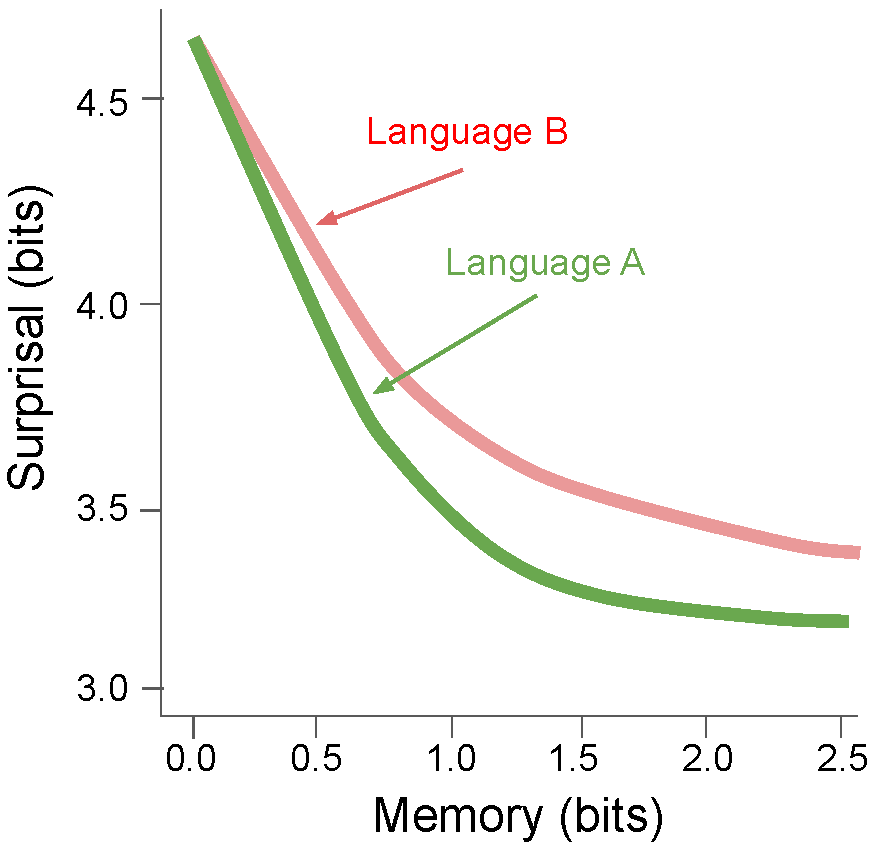
\includegraphics[width=0.5\textwidth]{figures/tradeoff.pdf} & \textcolor{red}{TODO visualize AUC here}
    \end{tabular}
    \caption{\textit{Left:} The memory-surprisal tradeoff in two hypothetical languages: In order to achieve a given level of surprisal, a comprehender has to invest a certain amount of memory resources, which can be quantified information-theoretically in terms of bits. In this case, Language A provides a more efficient tradeoff because comprehenders can achieve lower surprisal than Language B with the same  memory load.
    \textit{Right:} The Area under the Curve (AUC) for the two hypothetical languages. Language A has a lower AUC than Language B, corresponding to a more efficient memory-surprisal tradeoff.}
    %\mhahn{my plan for this figure is (i) curves for two languages A,B to show that tradeoffs can differ in their efficiency, (ii) a simple visualization of how AUC captures efficiency, (iii) a visualiation of MI $I_t$, (iv) a visualization of how the tradeoff curve is estimated based on $I_t$., (v) some kind of illustration of how locality leads to more efficient tradeoffs}}
    \label{fig:tradeoff}
\end{figure}


To test this hypothesis, \citet{Hahn2020modeling} provide a method for estimating the memory-surprisal tradeoff from corpus data.
This method is based on the notion of mutual information \citep{cover2006elements}, which quantifies the amount of statistical association between two random variables. 
If $X, Z, Y$ are random variables, then the mutual information of $X$ and $Y$, conditioned on $Z$, is defined to be:
\begin{align}
\label{eq:mi}
   \operatorname{I}[X:Y|Z] &\equiv \sum_{x,y,z} P(x,y,z) \log \frac{P(x,y,z)}{P(x,z)P(y,z)}. % \text{ bits} \\
 %   %\nonumber
 %   %&= \operatorname{H}[X,Z] - \operatorname{H}[X,Y,Z] \\
 %   %\nonumber
 %   %&= \operatorname{H}[Y,Z] - \operatorname{H}[Y,X,Z].
\end{align}
The key quantity derived from this is the mutual information between elements (such as morphemes) that are some distance $t$, conditioned on the intervening elements:
\begin{equation*}
    I_t \equiv \operatorname{I}[w_t : w_0 | w_1, \dots, w_{t-1}].
\end{equation*}
%This is visualized in Figure~\ref{fig:tradeoff} (left): $I_t$ This quantifies how much predictive information the element $t$ steps into the past provides about the next element, on average across all sequences in the language.
Based on this notion, \citet{Hahn2020modeling}  prove a bound on the memory-surprisal tradeoff:
%\mhahn{QUESTION: I'm wondering whether it is necessary to explain the theorem formally, or whether there might be a benefit in being a bit less formal here and only doing a pictorial presentation, referring to the PsychReview paper for the formal detai;s.}
%\begin{thm}\label{prop:suboptimal}(Information locality bound, \citet{Hahn2020modeling})
Assume that a comprehender's memory capacity is bounded as follows, for some positive integer $T$:
%For any positive integer $T$, let $M$ be a memory encoding function such that
\begin{equation}
\label{eq:memory-bound}
\operatorname{H}[m_t] \le \sum_{t=1}^T t I_t.
\end{equation}
Then we have a lower bound on the average surprisal $S_M$ experienced by that comprehender:
\begin{equation}
\label{eq:surprisal-bound}
S_M \ge S_\infty + \sum_{t=T+1}^\infty I_t.
\end{equation}
where $S_\infty$ is the average surprisal that would be achieved with perfectly veridical memory representations.

Because $I_t$ can be estimated from text data, this result yields a method for estimating a bound on the tradeoff curve from text data.


\citet{Hahn2020modeling} show that tradeoffs are more efficient when pairs of elements with higher mutual information are ordered close together, a property they refer to as \textsc{Information Locality}.
They argue that this information-theoretic notion of locality derives a range of locality principles proposed in the linguistic literature, such as the idea that syntactically related words tend to be close in linear distance \citep{rijkhoff-word-1986, hawkins1994performance, futrell-cross-linguistic-2015, liu-dependency-2017, temperley-minimizing-2018}.
Beyond providing evidence that word orders provide efficient tradeoffs, they also provide preliminary evidence that it accounts for some properties of morpheme ordering, using data of verb inflection in two languages (Japanese and Sesotho).
%and formalizes \citet{bybee-morphology-1985}'s idea that morphemes are closer together when they are more relevant to each other.

In this work, we aim to test the Efficient Tradeoff Hypothesis as a predictor of morpheme ordering more broadly, using data from more languages and from different parts of speech.
That is, we test whether morpheme ordering is more efficient than most other possible ways of ordering morphemes, and whether this accounts for the universal tendencies documented in Sections~\ref{sec:univ-nouns}--\ref{sec:univ-verbs}.

We review connections between the Efficient Tradeoff Hypothesis and previous theories of morpheme ordering in Section~\ref{sec:discussion}.

%\end{thm}
%Figure~\ref{fig:tradeoff} (right) visualizes a key consequence of this theorem, namely an information-theoretic notion of locality called Information locality:
%Orderings optimize this tradeoff when elements with high mutual information are closer together.

%Information locality has had success as a predictor of word order \citep{futrell2019information}, in particular for universals of the order inside noun phrases \citep{culbertson2020from,hahn-information-theoretic-2018,DBLP:conf/acl/FutrellDS20}.


%\becky{I think it's not 100\% clear to me how the memory-surprisal theory differs from previous work on locality that used memory and processing. Did they not use surprisal?} \jd{agreed that the intro (section 1) should include a little more info on similarities and differences in processing theories}



\section{Testing the Efficient Tradeoff Hypothesis}\label{seq:testing}
%\jd{...or modify the heading in a different way that clearly marks what's happening in the study (i think you don't set up the efficient tradeoff hypothesis in this paper)}

%\jd{include more signposting here: be clear about the overall research strategy (no more than 3 sentences telling reader what to expect), instead of making the reader reconstruct it by reading the next three sections}


We test the Efficient Tradeoff Hypothesis as a predictor of morpheme ordering.
To this end, we evaluate whether real orderings of morphemes lead to more efficient tradeoffs than most other possible orderings, and, whether the properties of real orderings arise from optimizing for the tradeoff's efficiency.

\subsection{Methods} 

\subsubsection{Data} 
We selected data from languages that have rich agglutinative morphology, that is, languages in which (i) verbs and nouns often have more than two morphemes per words, as that allows us to test predictions about the relative ordering of different morphemes, and (ii) the morphemes within a word have clearly delimited boundaries, providing unambiguous information about the ordering of morphemes.
Beyond the languages studied in \citet{Hahn2020modeling}, we obtained data from four such languages: the Universal Dependencies (UD) corpora for Korean \citep{chun2018building}, Turkish \citep{turkish-imst}, Hungarian \citep{hungarian-szeged}, and Finnish \citep{UDFinnish-TDT}.
In addition, we also reanalyze the data from \citet{Hahn2020modeling}, covering UD data for Japanese \citep{asahara2018universal} and the Child Language Data Exchange System (CHILDES) Sesotho corpus \citep{demuth1992acquisition} in a way consistent with our analysis of the other four languages.
We obtained between 7,328 (Hungarian) and 50,691 (Finnish) inflected nouns and between 2,735 (Hungarian) and 109,323 (Korean) inflected verbs in each language.


% Mutual information depends on the frequencies at which different morphological forms are used. We thus selected agglutinative languages for which large-scale text corpora with morphological annotation was available.




For nouns, we focused on Turkish, Hungarian, and Finnish, as nouns in these languages often have more than one affix.
We used all six languages for verbs.

For each language, we selected nouns and verbs based on the part-of-speech annotation in each corpus.
We treated adjectives together with nouns in Hungarian, Finnish, and Turkish, and together with verbs in Korean and Japanese.

We used available corpus annotation together with the grammatical literature on each language to determine which morphemes each extracted word was composed of (see SI Appendix, Section S1 for details).



\subsubsection{Estimating memory-surprisal tradeoffs}

In order to estimate memory-surprisal tradeoffs, we model words as strings of morphemes, following \citet{Hahn2020modeling}.
For instance, we represent \textit{juttu-i-hi-si} `into your stories' (Figure \ref{fig:noun-inflection}) as juttu-\textsc{Plural}-\textsc{Illative}-\textsc{2sgPoss}.
(See SI Appendix Section X for experiments taking morphophonological interactions between morphemes into account.)

For each language, we parameterize possible morpheme orderings through the $N!$ possible orderings of the $N$ affix slots.
Applying any such ordering to the forms extracted from the corpus results in a set of counterfactual forms with some associated memory-surprisal tradeoff curve.

%in particular, applying the real orderings (Figure \ref{tab:examples-verbs}) results in the actual morpheme sequences as found in the corpus.\jd{isn't this redundant/trivially true? ie is this saying more than "the real order is the real order"?}

We compare the real orderings (\textit{real}) to four different kinds of alternative orderings: randomized morpheme orderings (\textit{random}), random morpheme orderings that respect the universals discussed in Section \ref{sec:univ} (\textit{universals})\footnote{In addition to the two universals discussed there, they also respect the universal that derivational affixes are closer to the stem than inflectional affixes mentioned in the introduction.}, the reversed real orderings (\textit{reverse}), and morpheme orderings that are optimized to minimize AUC under the tradeoff curve (\textit{optimized}).  We estimated memory-surprisal tradeoffs and computationally optimized orderings for the AUC under the tradeoff curve using the method described in \citet{Hahn2020modeling}.

%\becky{I don't think the connection between MI and AUC was made super explicit earlier, so I guess that's why we're not saying ``optimized to maximize MI" ? I think the use of MI in this paper is not clear.}

If the Efficient Tradeoff Hypothesis accounts for morpheme ordering, then we expect that real orderings are more efficient than most other possible orderings, and close to the most efficient possible orderings.
We also expect that optimized orderings largely match the real orderings, to a higher degree than most other possible orderings.
If the Efficient Tradeoff Hypothesis predicts morpheme order even beyond the two universals, then real orderings should be more efficient even than most other orderings respecting the universals, and optimized orderings should resemble real orderings more than most other orderings respecting the universals.

%\jd{great, but why? why are we comparing real orderings to alternatives? and why these alternatives? ie, what will we learn by doing this? and/or what are the predictions? and do these predictions differ from those of alternative accounts put forth in the literature?}



%\subsection{Nouns}
%\mhahn{Here is an idea for how we might structure this section: We can describe the systems in the individual languages in prose and in broad strokes here, highlighting what's common and what's different across languages. For the nouns, it's interesting to point out that the relative position of Case and Possessor differs between Finnish and the rest, whereas the position of Number is stable. For the verbs, the discussion could refer to Table~\ref{tab:examples-verbs}. I've collapsed all the Tense/Aspect/Modality/Negation morphemes into one big category ``TAM, Polarity'' since aligning the morphemes in each language with those individual categories seems very hard, and in any case there are differences between the languages. Talking about this in broad strokes, again highlighting parallels and differences, should be the right level of detail here. You can draw on Table S1 and Tables S5, S12, S13 in the appendix for my revised verb morpheme segmentation in Korean, Turkish, and Hungarian. We can then leave precise and detailed discussion of each of the languages, including detailed references to the literature for these individual languages, to the appendix. The \texttt{enumerate} blocks could go into the appendix, with some description of what each morpheme does and references to reference grammars (I can do this).}
%We're interested in investigating languages where nouns are inflected with multiple suffixes, because that allows us to more extensively measure the relationship between mutual information and mutual information. As such, we only investigated our hypothesis on Turkish, Hungarian, and Finnish nouns. All of these languages inflect nouns for number, possessor person, possessor number, and case, in that order. Finnish is the exception, where we include derivation (verbs that are nominalized, for example), and where the possessor person and number appears after the case suffix in the natural ordering. 
%In contrast, the number suffix, which is generally only marked for the plural, has a stable position close to the root in all three languages. Number has high mutual information with the noun root, because certain nouns have a tendency to appear only in the plural or only in the singular. As such, number must come close to the root.
%\subsection{Verbs}
%For verbs, we investigated Finnish, Hungarian, Japanese, Korean, Sesotho, and Turkish inflectional suffixes. Broadly speaking, all of the languages have a real ordering of valence, voice, negation, tense/aspect/mood (TAM), person and number, and formality, where applicable. \becky{TODO: Check that this is correct and discuss some specifics.} 
%\becky{Which language provides data for which kind of suffix?}
%Following \citet{Hahn2020modeling}, we compare the efficiency each natural language's morpheme orderings (\textit{real}) to three different kinds of baselines: randomized morpheme orderings (\textit{random}), the reversed natural orderings (\textit{reverse}), and morpheme orderings that are optimized to maximize MI (\textit{optimized}). 


%https://en.wiktionary.org/wiki/%EB%B0%94%EB%9D%BC%EB%8B%A4

\subsection{Results}

Figures \ref{fig:auc_verbs} and \ref{fig:auc_nouns} show area under the curve (AUC) plots for random orders as compared to the real order of morphemes for verbs and nouns, respectively.
%Here, AUC refers to the area under the curve for the memory-surprisal tradeoff for each order, where the lower the AUC is, the more efficient that memory-surprisal tradeoff is.
In most languages, real orderings have lower AUC than the vast majority of random baseline orderings, including the baselines that satisfy the universals. This is true for both nouns and verbs. In fact, the AUC of real orderings was so similar to the AUC of computationally optimized orderings that the two are visually indistinguishible in Figure  \ref{fig:auc_nouns}. This suggests that real morpheme orderings enable more efficient memory-surprisal tradeoffs than most of the $N!$ possible orderings.
Finnish verbs form the only exception; AUCs of real orderings are similar to those of baseline orderings (see below for discussion).

Second, we evaluated the accuracy of optimized orderings in predicting real orderings.
If the Efficient Tradeoff Hypothesis predicts morpheme order, then optimized orderings should achueve a higher prediction accuracy than most other possible orderings.
Figures \ref{tab:optimized_acc_nouns}--\ref{tab:optimized_acc_verbs} show the accuracy of optimized and random baseline orderings in predicting real orderings. 
We measured accuracy by counting what fraction of all pairs of affixes within a single word from the corpus are ordered in the same relative order as under the real order (see SI Section X for other ways of quantifying accuracy).
%We defined three measures of agreement:
%\textit{Pairs} counts what fraction of all pairs of affixes within a single word from the corpus are ordered in the same relative order under both orderings.
%\textit{Full} counts what fraction of words from the corpus is ordered entirely identically under both orderings.
%Finally, \textit{Full (Types)} is analogous to \textit{Full} but only counts words that appear multiple times only once, in order to control for the possible effect of individual highly frequent forms.


For nouns, the accuracy of optimized orderings is perfect, far above the agreement with random grammars.
For verbs, accuracy of optimized orderings is above 90\% for Hungarian, Turkish, Korean, Japanese, and Sesotho prefixes, better than at least 80\% of the baseline grammars. 
With the exception of Hungarian (where the universals almost fully determine the ordering), optimized orderings also match real orders better than almost all other orderings that satisfy the universals.
For Finnish and Sesotho suffixes, agreement is lower, though still at 84\% (Finnish) and 78\% (Sesotho), compared to an average of 57\% (Finnish) or 46\% (Sesotho) for random baselines.

Figures \ref{fig:real_and_optimized_nouns} and \ref{fig:real_and_optimized_verbs} directly compare real and optimized orderings for nouns and verbs respectively.
The real and optimized noun orders show a perfect match.
In particular, Greenberg's Universal 39 is recovered by all optimized orderings.
Beyond this, optimized orderings also recover the language-specific ordering of possessive suffuxes (before the number marker in Finnish, after it in Turkish and Hungarian).

For verbs, real and verb optimized orders show some disagreement in each language.
Comparing the universal verb morpheme ordering to the optimized ordering for each language, Hungarian, Japanese, Korean, and Sesotho (suffixes and prefixes) match the universal ordering perfectly for the morphemes occurring in each of these languages. 
Turkish matches the universal order except for the 3rd person plural agreement marker ``-lar-'', which is separated from the other agreement morphemes in both real and optimized orderings.
For Finnish, the optimized order is the same as the universal order except for the fact that the agreement marker comes closest to the root instead of furthest, which accounts for the reduced accuracy observed in Figure~\ref{tab:optimized_acc_verbs}.
This can be traced to a crosslinguistically uncommon peculiarity of the Finnish passive, which uses a single agreement marker that is only used for passives, and which does not distinguish between person and number categories (referred to as impersonal by \citet[Section 69]{karlsson1999finnish}).
This means that the agreement marker has substantial mutual information with the voice morpheme, and optimized orderings prefer agreement and voice morphemes to be adjacent.
On active forms -- which, unlike the passive, are fully inflected for person and number -- optimized orderings place the agreement slot after the TAM slot, in agreement with the real ordering.

%\mhahn{what would the random accuracy be in predicting?}



%Taking a step back and looking at all of these languages at a whole, we see that the languages' optimized orders tend to closely mirror Bybee's universal ordering, which also means that these languages also have a high level of agreement between them on the relative ordering of verbal morphemes. As such, it's possible to predict Bybee's universal ordering from looking at commonalities between optimized orders of natural languages. 


%\mhahn{TODO make clear that we are explaining the universals and language-specific patterns beyond those}

%\becky{conclude}


\definecolor{optimized}{HTML}{F8766D}
\definecolor{random}{HTML}{A3A500}
\definecolor{real}{HTML}{00BF7D}
\definecolor{reverse}{HTML}{00B0F6}
\definecolor{universals}{HTML}{E76BF3}


\begin{figure}
\begin{center}
\begin{tabular}{ccc}
\textsc{Finnish} & \textsc{Turkish} & \textsc{Hungarian} \\
    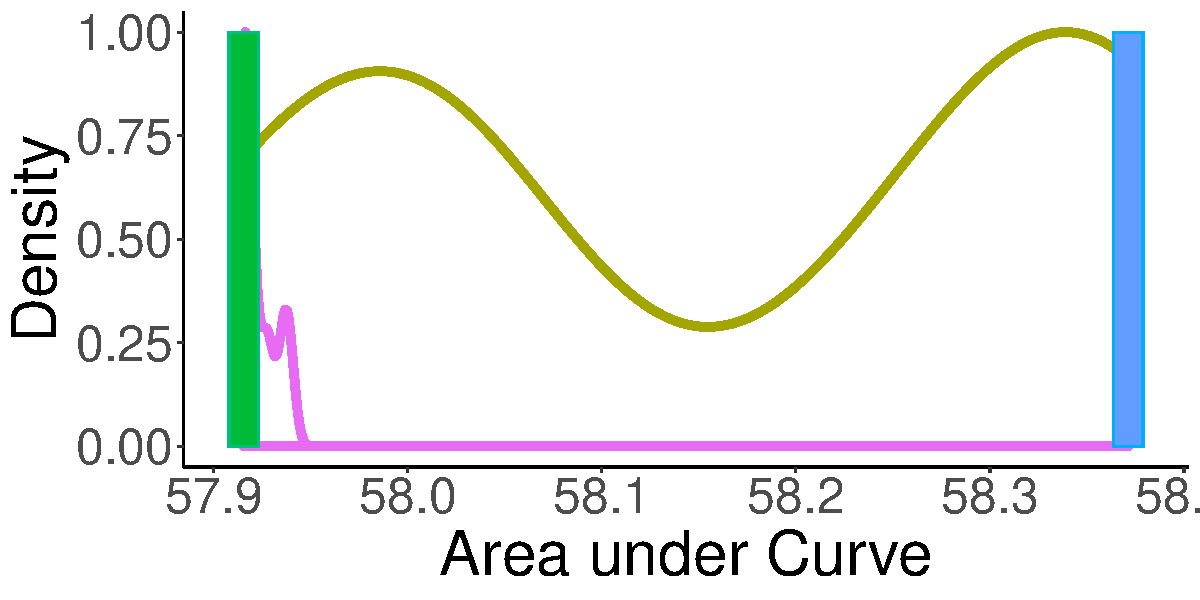
\includegraphics[width=0.3\textwidth]{figures/finnish_nouns/suffixes-byMorphemes-auc-hist-heldout-Coarse-FineSurprisal-optimized.pdf}
    &
    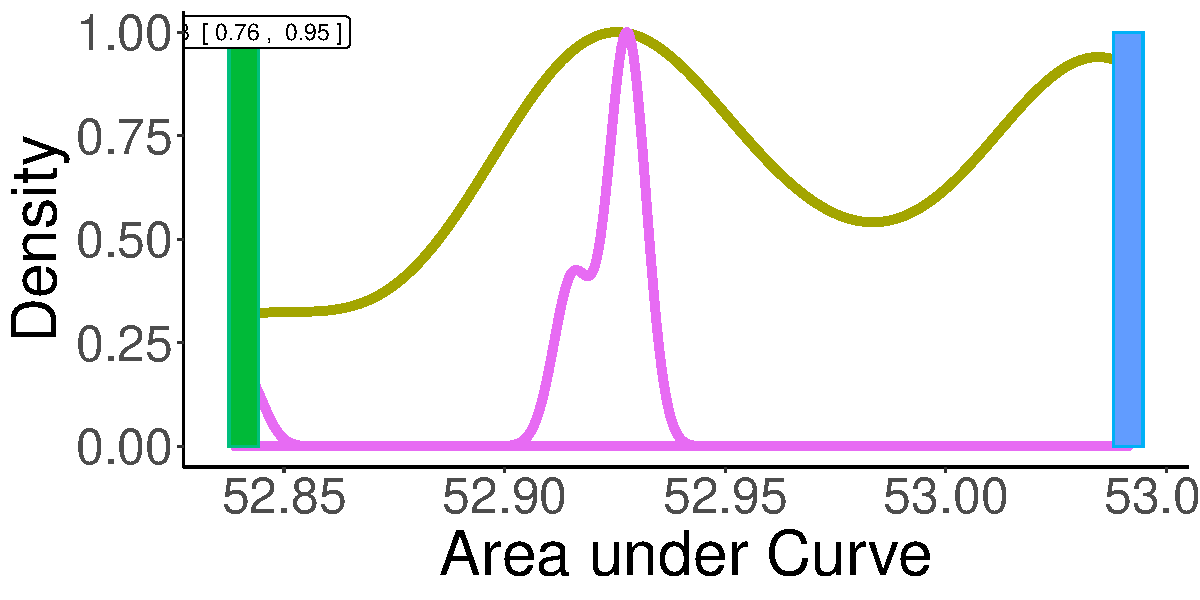
\includegraphics[width=0.3\textwidth]{figures/turkish_nouns/suffixes-byMorphemes-auc-hist-heldout-Coarse-FineSurprisal-optimized.pdf}
    &
    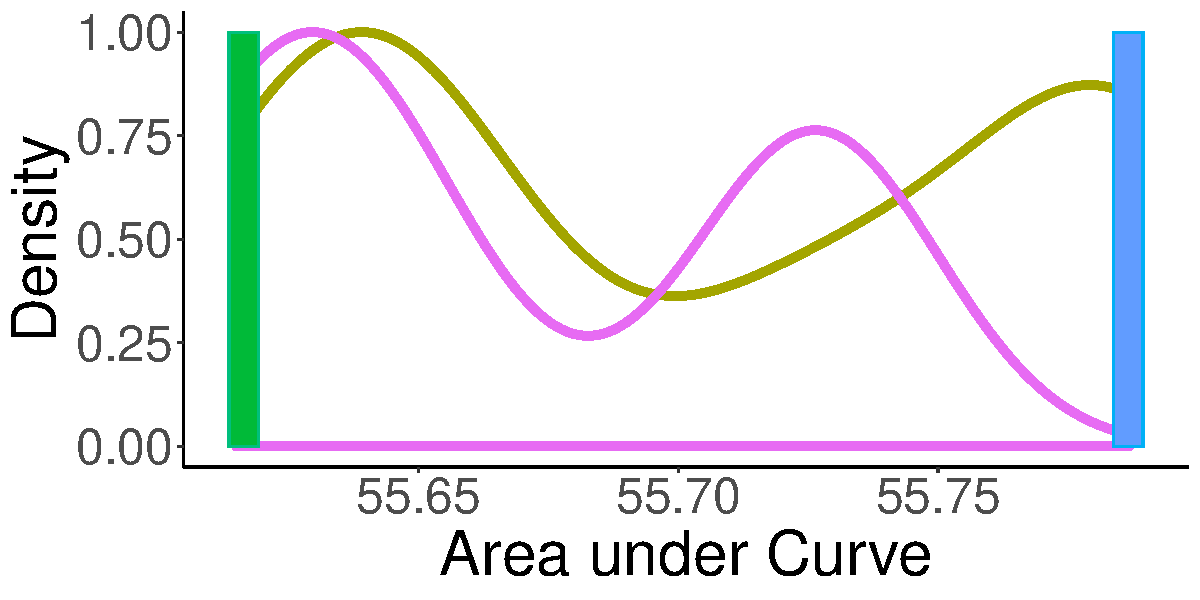
\includegraphics[width=0.3\textwidth]{figures/hungarian_nouns/suffixes-byMorphemes-auc-hist-heldout-Coarse-FineSurprisal-optimized.pdf}
    \end{tabular}
    
    \begin{tabular}{llllllll}
\textbf{\textcolor{real}{----}} Real&
\textbf{\textcolor{random}{----}} Random&
\textbf{\textcolor{universals}{----}} Universals&
\textbf{\textcolor{reverse}{----}} Reverse
\end{tabular}
\end{center}
    
    \caption{AUC Histograms for Noun Suffixes: We show smoothed histograms of baseline orderings (brown) and orderings satisfying the universals (purple), and the AUC values for real (green) and reverse (blue) orderings. For the real orderings, we also indicate what fraction of baseline grammars have higher AUC, with a binomial confidence interval. Optimizesd orderings are identical to real orderings in this figure, and thus not plotted.  }
    \label{fig:auc_nouns}
\end{figure}

\begin{figure}
    \begin{center}
    \begin{tabular}{cccccc}
    \textsc{Finnish} & \textsc{Turkish} & \textsc{Hungarian} \\
        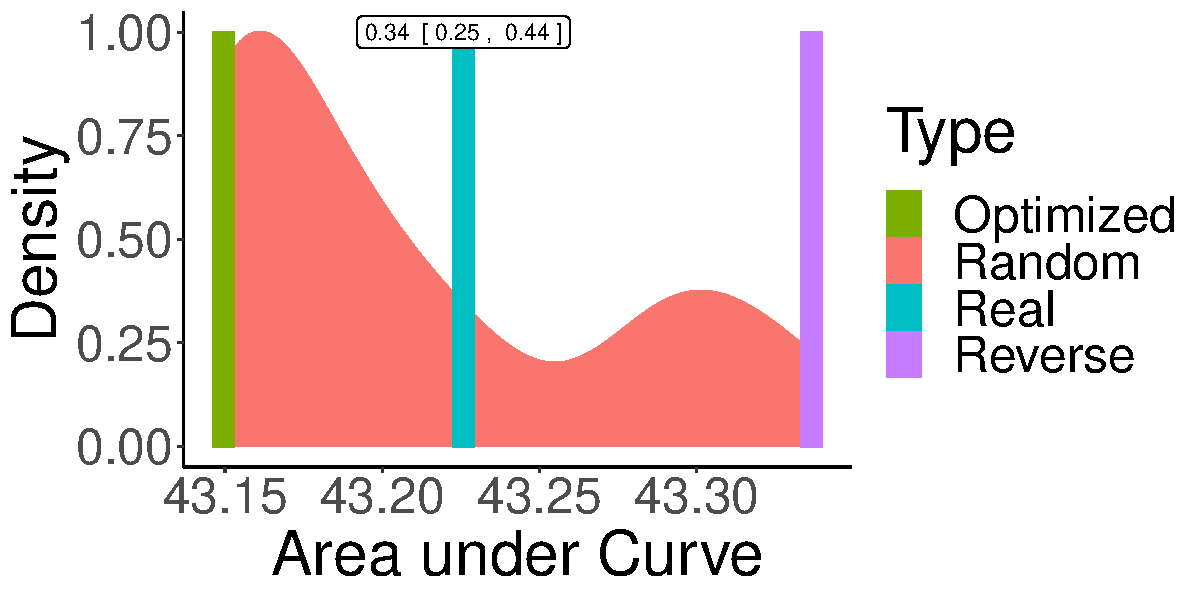
\includegraphics[width=0.3\textwidth]{figures/finnish_verbs/suffixes-byMorphemes-auc-hist-heldout-Coarse-FineSurprisal-optimized.pdf}
        &
    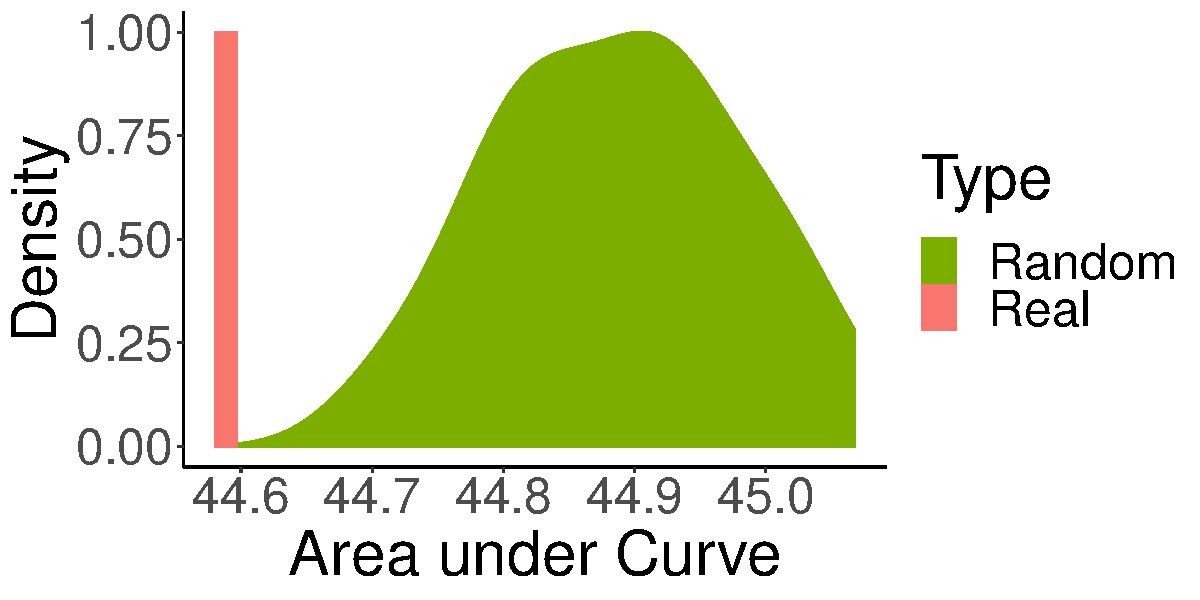
\includegraphics[width=0.3\textwidth]{figures/turkish_verbs/suffixes-byMorphemes-auc-hist-heldout-Coarse-FineSurprisal-optimized.pdf}
    &
    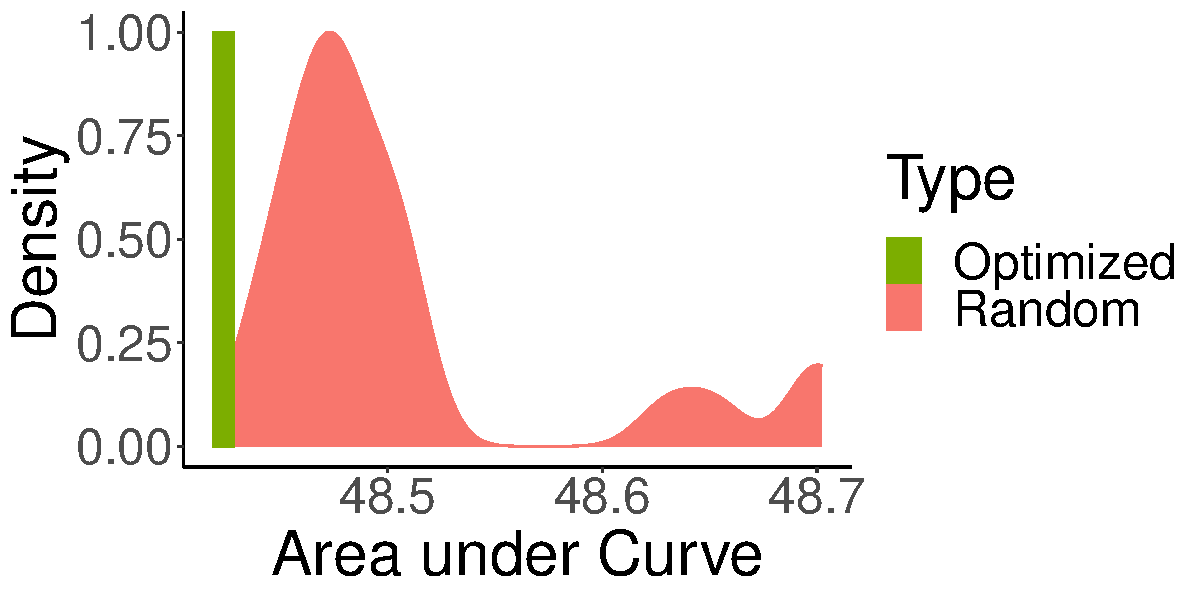
\includegraphics[width=0.3\textwidth]{figures/hungarian_verbs/suffixes-byMorphemes-auc-hist-heldout-Coarse-FineSurprisal-optimized.pdf}
    \\
    \textsc{Korean} & \textsc{Japanese} & \textsc{Sesotho Prefixes} \\
    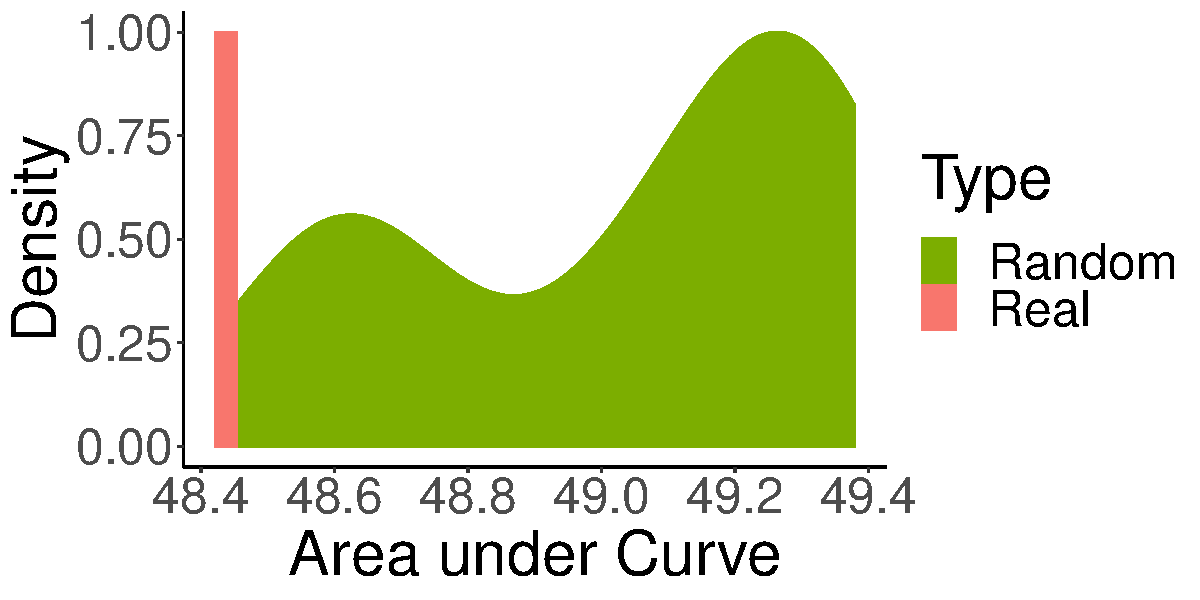
\includegraphics[width=0.3\textwidth]{figures/korean/suffixes-byMorphemes-auc-hist-heldout-Coarse-FineSurprisal-optimized.pdf}
    &
        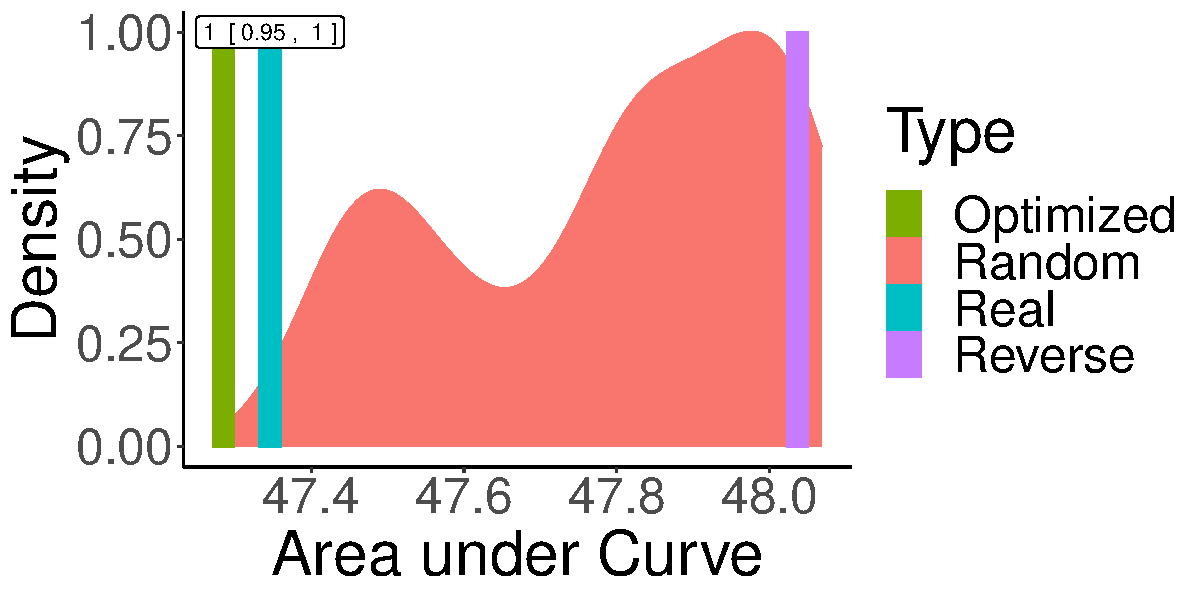
\includegraphics[width=0.3\textwidth]{figures/japanese/suffixes-byMorphemes-auc-hist-heldout-Coarse-FineSurprisal-optimized.pdf}
        &
            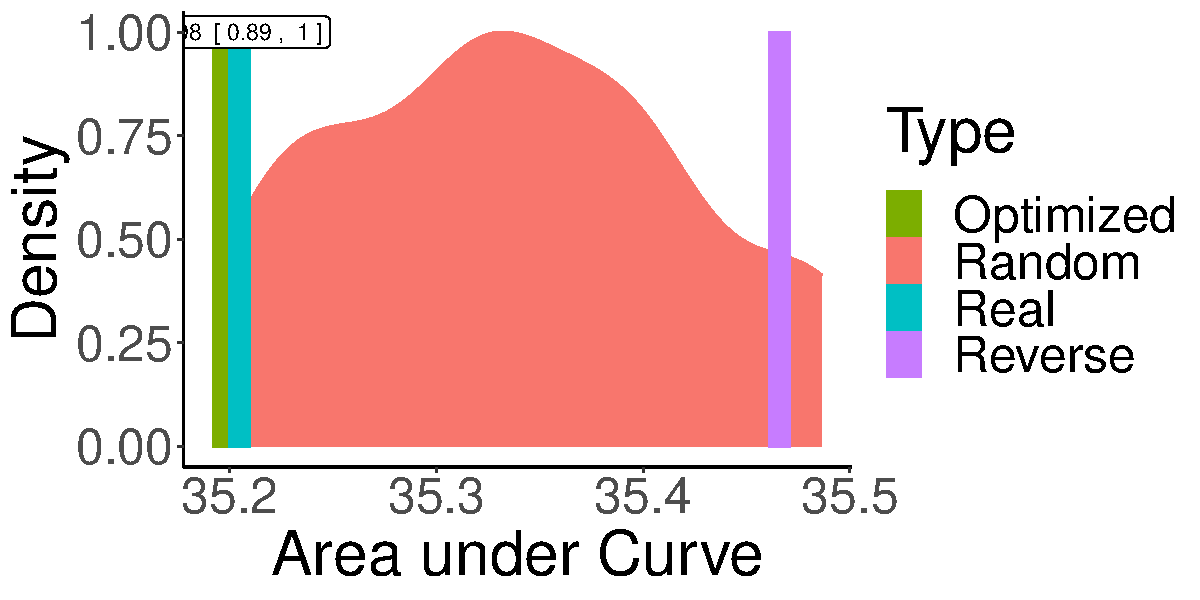
\includegraphics[width=0.3\textwidth]{figures/sesotho_prefixes/suffixes-byMorphemes-auc-hist-heldout-Coarse-FineSurprisal-optimized.pdf}
            \\
            \textsc{Sesotho Suffixes} \\
            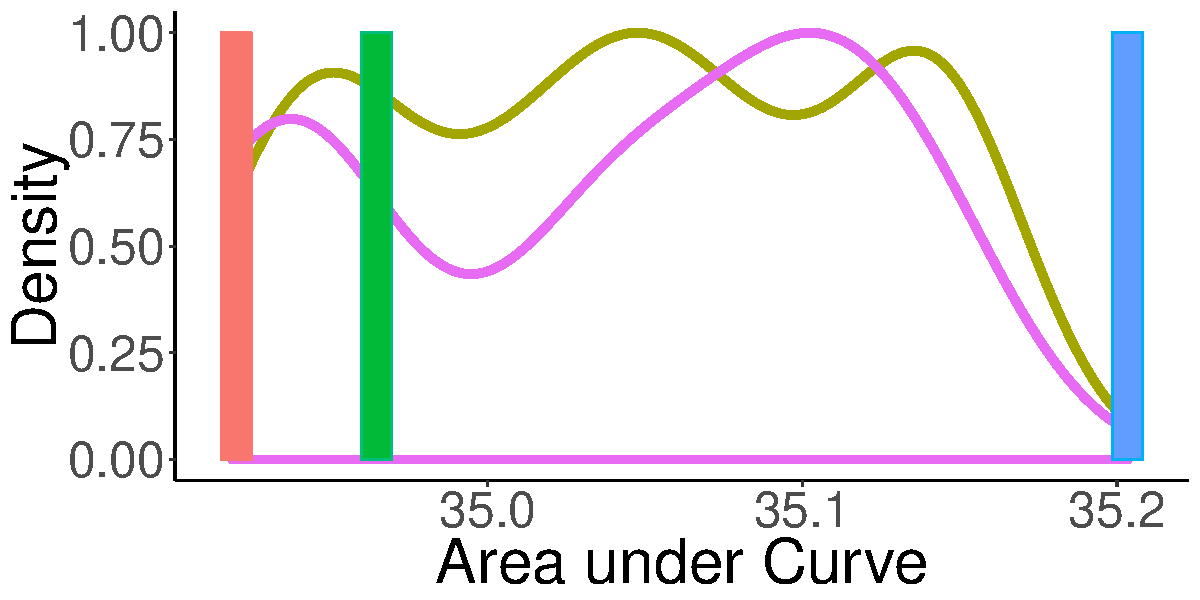
\includegraphics[width=0.3\textwidth]{figures/sesotho_suffixes/suffixes-byMorphemes-auc-hist-heldout-Coarse-FineSurprisal-optimized.pdf}
    \end{tabular}

    \begin{tabular}{llllllll}
\textbf{\textcolor{real}{----}} Real&
\textbf{\textcolor{optimized}{----}} Optimized&
\textbf{\textcolor{random}{----}} Random&
\textbf{\textcolor{universals}{----}} Universals&
\textbf{\textcolor{reverse}{----}} Reverse
\end{tabular}
    \end{center}
    \caption{AUC Histograms for Verb Affixes: We show smoothed histograms of baseline orderings (brown) and orderings satisfying the universals (purple), and the AUC values for optimized (red), real (green), and reverse (blue) orderings. For the real orderings, we also indicate what fraction of baseline grammars have higher AUC, with a binomial confidence interval.}
    \label{fig:auc_verbs}
\end{figure}


\begin{figure}[]
    \centering
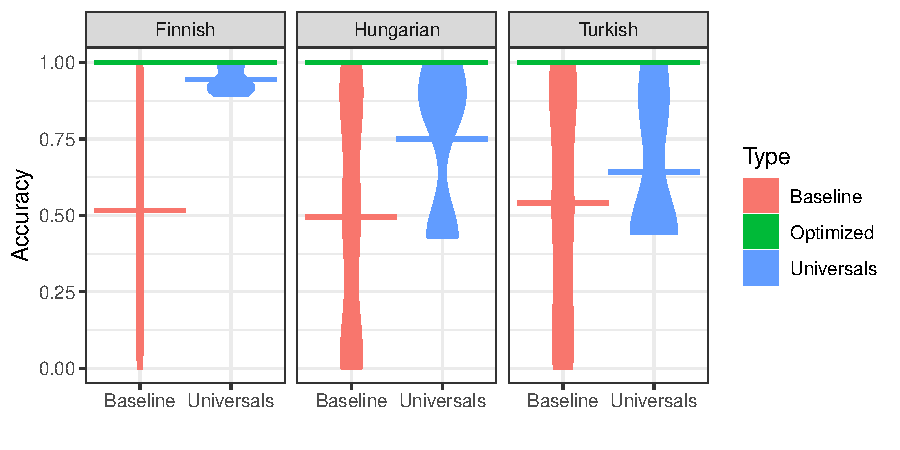
\includegraphics[width=0.7\textwidth]{figures/accuracies_nouns.pdf}
    \caption{Accuracies in predicting noun morpheme ordering.
    Optimized orderings achieve perfect accuracy, indicated by the red bars at the top.
    For the baselines, we provide both smoothed violin plots of the distribution of accuracies, and horizontal lines indicating mean accuracies.
    Random baselines have a mean accuracy of about 50\%; baselines respecting the universals tend to have higher accuracy, though mostly not as high as the optimized ordering.
    Comparisons between optimized and baseline (both random and based on universals) orderings are significant at $p<0.001$.}
    \label{tab:optimized_acc_nouns}
\end{figure}

\begin{figure}[]
    \centering
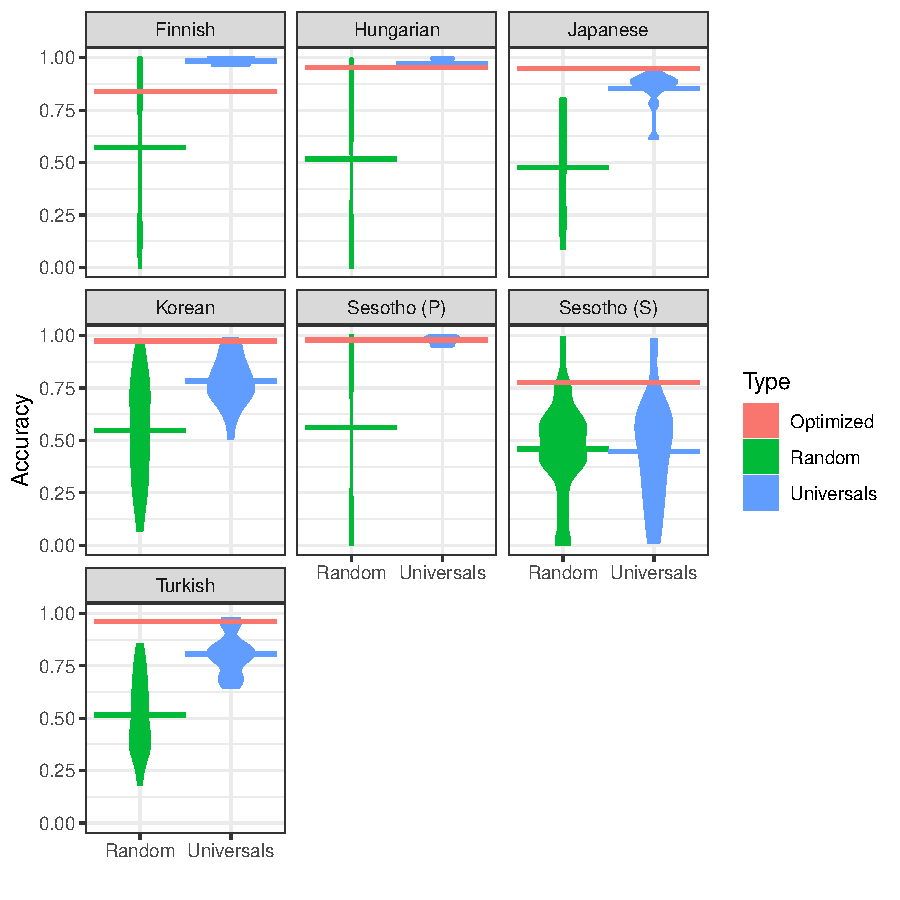
\includegraphics[width=0.8\textwidth]{figures/accuracies_verbs.pdf}
    \caption{Accuracies in predicting verb morpheme ordering.
    For the baselines, we provide both a smoothed violin plot of the distribution of accuracies, and the mean accuracy as a horizontal line (green and blue). For the optimized order, we show the accuracy as a horizontal line (red).
    In all languages, optimized orderings provide higher accuracy than the mean of the random baselines ($p<0.001$).}
    \label{tab:optimized_acc_verbs}
\end{figure}

    %`Pairs' indicates the fraction of pairs of morphemes occurring together in the same word that are ordered correctly. `Full' indicates the fraction of verb forms in the corpus that are ordered fully correctly. `Full (Types)' counts forms that occur multiple times only once, it thus down-weights the role of frequent forms.

\begin{figure}[]
\begin{tabular}{cccccccc}
\textsc{Turkish} & \textsc{Hungarian} & \textsc{Finnish} \\
\begin{minipage}{.3\textwidth}
    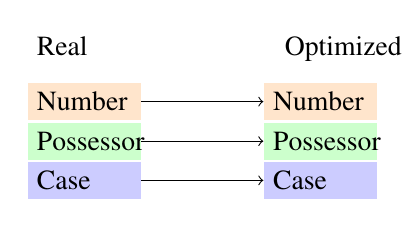
\begin{tikzpicture}[%
% common options for blocks:
block/.style = {draw, fill=blue!30, align=center, anchor=west,
            minimum height=0.65cm, inner sep=0},
% common options for the circles:
ball/.style = {circle, draw, align=center, anchor=north, inner sep=0}]
\node[rectangle,text width=1.2cm,anchor=base] (A0) at (1,-0.3) {Real};
\node[rectangle,text width=0.9cm,anchor=base] (B0) at (4,-0.3) {Optimized};
\node[rectangle,text width=1.2cm,anchor=base, fill=orange!20] (A1) at (1,-1.0) {Number};
\node[rectangle,text width=1.2cm,anchor=base, fill=green!20] (A2) at (1,-1.5) {Possessor};
\node[rectangle,text width=1.2cm,anchor=base, fill=blue!20] (A3) at (1,-2.0) {Case};
\node[rectangle,text width=1.2cm,anchor=base, fill=orange!20] (B1) at (4,-1.0) {Number};
\node[rectangle,text width=1.2cm,anchor=base, fill=green!20] (B2) at (4,-1.5) {Possessor};
\node[rectangle,text width=1.2cm,anchor=base, fill=blue!20] (B3) at (4,-2.0) {Case};
\draw[->] (A1.east) to (B1.west);
\draw[->] (A2.east) to (B2.west);
\draw[->] (A3.east) to (B3.west);
\end{tikzpicture}

    \end{minipage}
  &
  \begin{minipage}{.3\textwidth}
    \begin{tikzpicture}[%
% common options for blocks:
block/.style = {draw, fill=blue!30, align=center, anchor=west,
            minimum height=0.65cm, inner sep=0},
% common options for the circles:
ball/.style = {circle, draw, align=center, anchor=north, inner sep=0}]
\node[rectangle,text width=1.2cm,anchor=base] (A0) at (1,-0.3) {Real};
\node[rectangle,text width=0.9cm,anchor=base] (B0) at (4,-0.3) {Optimized};
\node[rectangle,text width=1.2cm,anchor=base] (A1) at (1,-1.0) {Number};
\node[rectangle,text width=1.2cm,anchor=base] (A2) at (1,-1.5) {Psor_person};
\node[rectangle,text width=1.2cm,anchor=base] (A3) at (1,-2.0) {Psor_number};
\node[rectangle,text width=1.2cm,anchor=base] (A4) at (1,-2.5) {Case};
\node[rectangle,text width=1.2cm,anchor=base] (B1) at (4,-1.0) {Number};
\node[rectangle,text width=1.2cm,anchor=base] (B2) at (4,-1.5) {Psor_person};
\node[rectangle,text width=1.2cm,anchor=base] (B3) at (4,-2.0) {Psor_number};
\node[rectangle,text width=1.2cm,anchor=base] (B4) at (4,-2.5) {Case};
\draw[->] (A1.east) to (B1.west);
\draw[->] (A2.east) to (B2.west);
\draw[->] (A3.east) to (B3.west);
\draw[->] (A4.east) to (B4.west);
\end{tikzpicture}

    \end{minipage}
  &
  \begin{minipage}{.3\textwidth}
    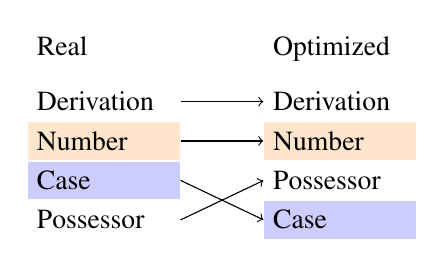
\begin{tikzpicture}[%
% common options for blocks:
block/.style = {draw, fill=blue!30, align=center, anchor=west,
            minimum height=0.65cm, inner sep=0},
% common options for the circles:
ball/.style = {circle, draw, align=center, anchor=north, inner sep=0}]
\node[rectangle,text width=1.7cm,anchor=base] (A0) at (1,-0.3) {Real};
\node[rectangle,text width=1.7cm,anchor=base] (B0) at (4,-0.3) {Optimized};
\node[rectangle,text width=1.7cm,anchor=base] (A1) at (1,-1.0) {Derivation};
\node[rectangle,text width=1.7cm,anchor=base, fill=orange!20] (A2) at (1,-1.5) {Number};
\node[rectangle,text width=1.7cm,anchor=base, fill=blue!20] (A3) at (1,-2.0) {Case};
\node[rectangle,text width=1.7cm,anchor=base] (A4) at (1,-2.5) {Possessor};
\node[rectangle,text width=1.7cm,anchor=base] (B1) at (4,-1.0) {Derivation};
\node[rectangle,text width=1.7cm,anchor=base, fill=orange!20] (B2) at (4,-1.5) {Number};
\node[rectangle,text width=1.7cm,anchor=base] (B3) at (4,-2.0) {Possessor};
\node[rectangle,text width=1.7cm,anchor=base, fill=blue!20] (B4) at (4,-2.5) {Case};
\draw[->] (A1.east) to (B1.west);
\draw[->] (A2.east) to (B2.west);
\draw[->] (A3.east) to (B4.west);
\draw[->] (A4.east) to (B3.west);
\end{tikzpicture}

  \end{minipage}
  \end{tabular}
  
    \caption{Real and optimized ordering (nouns). Colors indicate universal position slots relevant for Greenbergs' Universal 39.}
    \label{fig:real_and_optimized_nouns}
\end{figure}


\begin{figure}[]

\begin{tabular}{cccccccc}
\textsc{Turkish} & \textsc{Hungarian} & \textsc{Finnish} \\
\begin{minipage}{.3\textwidth}
    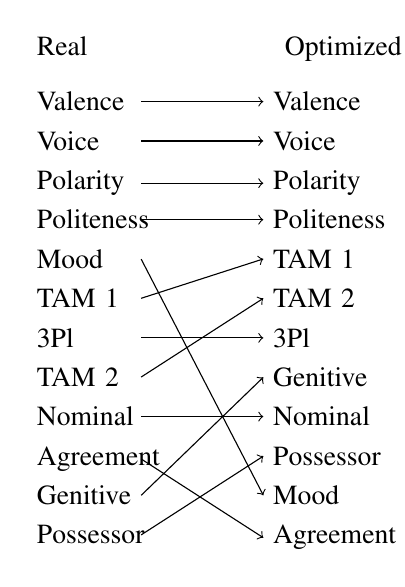
\begin{tikzpicture}[%
% common options for blocks:
block/.style = {draw, fill=blue!30, align=center, anchor=west,
            minimum height=0.65cm, inner sep=0},
% common options for the circles:
ball/.style = {circle, draw, align=center, anchor=north, inner sep=0}]
\node[rectangle,text width=1.2cm,anchor=base] (A0) at (1,-0.3) {Real};
\node[rectangle,text width=0.9cm,anchor=base] (B0) at (4,-0.3) {Optimized};
\node[rectangle,text width=1.2cm,anchor=base] (A1) at (1,-1.0) {Valence};
\node[rectangle,text width=1.2cm,anchor=base] (A2) at (1,-1.5) {Voice};
\node[rectangle,text width=1.2cm,anchor=base] (A3) at (1,-2.0) {Polarity};
\node[rectangle,text width=1.2cm,anchor=base] (A4) at (1,-2.5) {Politeness};
\node[rectangle,text width=1.2cm,anchor=base] (A5) at (1,-3.0) {Mood};
\node[rectangle,text width=1.2cm,anchor=base] (A6) at (1,-3.5) {TAM 1};
\node[rectangle,text width=1.2cm,anchor=base] (A7) at (1,-4.0) {3Pl};
\node[rectangle,text width=1.2cm,anchor=base] (A8) at (1,-4.5) {TAM 2};
\node[rectangle,text width=1.2cm,anchor=base] (A9) at (1,-5.0) {Nominal};
\node[rectangle,text width=1.2cm,anchor=base] (A10) at (1,-5.5) {Agreement};
\node[rectangle,text width=1.2cm,anchor=base] (A11) at (1,-6.0) {Genitive};
\node[rectangle,text width=1.2cm,anchor=base] (A12) at (1,-6.5) {Possessor};
\node[rectangle,text width=1.2cm,anchor=base] (B1) at (4,-1.0) {Valence};
\node[rectangle,text width=1.2cm,anchor=base] (B2) at (4,-1.5) {Voice};
\node[rectangle,text width=1.2cm,anchor=base] (B3) at (4,-2.0) {Polarity};
\node[rectangle,text width=1.2cm,anchor=base] (B4) at (4,-2.5) {Politeness};
\node[rectangle,text width=1.2cm,anchor=base] (B5) at (4,-3.0) {TAM 1};
\node[rectangle,text width=1.2cm,anchor=base] (B6) at (4,-3.5) {TAM 2};
\node[rectangle,text width=1.2cm,anchor=base] (B7) at (4,-4.0) {3Pl};
\node[rectangle,text width=1.2cm,anchor=base] (B8) at (4,-4.5) {Genitive};
\node[rectangle,text width=1.2cm,anchor=base] (B9) at (4,-5.0) {Nominal};
\node[rectangle,text width=1.2cm,anchor=base] (B10) at (4,-5.5) {Possessor};
\node[rectangle,text width=1.2cm,anchor=base] (B11) at (4,-6.0) {Mood};
\node[rectangle,text width=1.2cm,anchor=base] (B12) at (4,-6.5) {Agreement};
\draw[->] (A1.east) to (B1.west);
\draw[->] (A2.east) to (B2.west);
\draw[->] (A3.east) to (B3.west);
\draw[->] (A4.east) to (B4.west);
\draw[->] (A5.east) to (B11.west);
\draw[->] (A6.east) to (B5.west);
\draw[->] (A7.east) to (B7.west);
\draw[->] (A8.east) to (B6.west);
\draw[->] (A9.east) to (B9.west);
\draw[->] (A10.east) to (B12.west);
\draw[->] (A11.east) to (B8.west);
\draw[->] (A12.east) to (B10.west);
\end{tikzpicture}

  \end{minipage}
  &
  \begin{minipage}{.3\textwidth}
    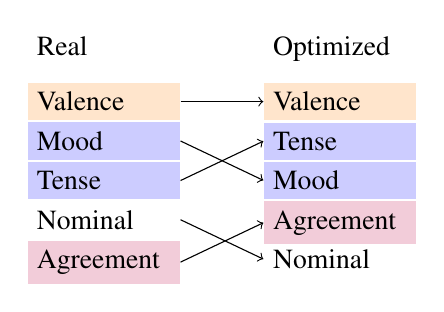
\begin{tikzpicture}[%
% common options for blocks:
block/.style = {draw, fill=blue!30, align=center, anchor=west,
            minimum height=0.65cm, inner sep=0},
% common options for the circles:
ball/.style = {circle, draw, align=center, anchor=north, inner sep=0}]
\node[rectangle,text width=1.7cm,anchor=base] (A0) at (1,-0.3) {Real};
\node[rectangle,text width=1.7cm,anchor=base] (B0) at (4,-0.3) {Optimized};
\node[rectangle,text width=1.7cm,anchor=base, fill=orange!20] (A1) at (1,-1.0) {Valence};
\node[rectangle,text width=1.7cm,anchor=base, fill=blue!20] (A2) at (1,-1.5) {Mood};
\node[rectangle,text width=1.7cm,anchor=base, fill=blue!20] (A3) at (1,-2.0) {Tense};
\node[rectangle,text width=1.7cm,anchor=base] (A4) at (1,-2.5) {Nominal};
\node[rectangle,text width=1.7cm,anchor=base, fill=purple!20] (A5) at (1,-3.0) {Agreement};
\node[rectangle,text width=1.7cm,anchor=base, fill=orange!20] (B1) at (4,-1.0) {Valence};
\node[rectangle,text width=1.7cm,anchor=base, fill=blue!20] (B2) at (4,-1.5) {Tense};
\node[rectangle,text width=1.7cm,anchor=base, fill=blue!20] (B3) at (4,-2.0) {Mood};
\node[rectangle,text width=1.7cm,anchor=base, fill=purple!20] (B4) at (4,-2.5) {Agreement};
\node[rectangle,text width=1.7cm,anchor=base] (B5) at (4,-3.0) {Nominal};
\draw[->] (A1.east) to (B1.west);
\draw[->] (A2.east) to (B3.west);
\draw[->] (A3.east) to (B2.west);
\draw[->] (A4.east) to (B5.west);
\draw[->] (A5.east) to (B4.west);
\end{tikzpicture}

  \end{minipage}
  &
    \begin{minipage}{.3\textwidth}
    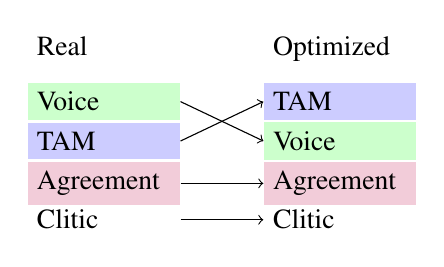
\begin{tikzpicture}[%
% common options for blocks:
block/.style = {draw, fill=blue!30, align=center, anchor=west,
            minimum height=0.65cm, inner sep=0},
% common options for the circles:
ball/.style = {circle, draw, align=center, anchor=north, inner sep=0}]
\node[rectangle,text width=1.7cm,anchor=base] (A0) at (1,-0.3) {Real};
\node[rectangle,text width=1.7cm,anchor=base] (B0) at (4,-0.3) {Optimized};
\node[rectangle,text width=1.7cm,anchor=base, fill=green!20] (A1) at (1,-1.0) {Voice};
\node[rectangle,text width=1.7cm,anchor=base, fill=blue!20] (A2) at (1,-1.5) {TAM};
\node[rectangle,text width=1.7cm,anchor=base, fill=purple!20] (A3) at (1,-2.0) {Agreement};
\node[rectangle,text width=1.7cm,anchor=base] (A4) at (1,-2.5) {Clitic};
\node[rectangle,text width=1.7cm,anchor=base, fill=blue!20] (B1) at (4,-1.0) {TAM};
\node[rectangle,text width=1.7cm,anchor=base, fill=green!20] (B2) at (4,-1.5) {Voice};
\node[rectangle,text width=1.7cm,anchor=base, fill=purple!20] (B3) at (4,-2.0) {Agreement};
\node[rectangle,text width=1.7cm,anchor=base] (B4) at (4,-2.5) {Clitic};
\draw[->] (A1.east) to (B2.west);
\draw[->] (A2.east) to (B1.west);
\draw[->] (A3.east) to (B3.west);
\draw[->] (A4.east) to (B4.west);
\end{tikzpicture}

  \end{minipage}
  \\
  \textsc{Korean}  & \textsc{Japanese} & \textsc{Sesotho Prefixes} \\
      \begin{minipage}{.3\textwidth}
    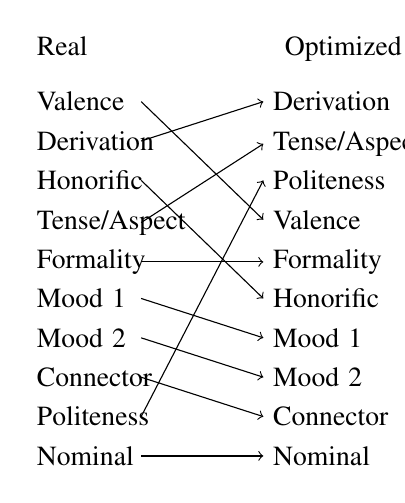
\begin{tikzpicture}[%
% common options for blocks:
block/.style = {draw, fill=blue!30, align=center, anchor=west,
            minimum height=0.65cm, inner sep=0},
% common options for the circles:
ball/.style = {circle, draw, align=center, anchor=north, inner sep=0}]
\node[rectangle,text width=1.2cm,anchor=base] (A0) at (1,-0.3) {Real};
\node[rectangle,text width=0.9cm,anchor=base] (B0) at (4,-0.3) {Optimized};
\node[rectangle,text width=1.2cm,anchor=base] (A1) at (1,-1.0) {Valence};
\node[rectangle,text width=1.2cm,anchor=base] (A2) at (1,-1.5) {Derivation};
\node[rectangle,text width=1.2cm,anchor=base] (A3) at (1,-2.0) {Honorific};
\node[rectangle,text width=1.2cm,anchor=base] (A4) at (1,-2.5) {Tense/Aspect};
\node[rectangle,text width=1.2cm,anchor=base] (A5) at (1,-3.0) {Formality};
\node[rectangle,text width=1.2cm,anchor=base] (A6) at (1,-3.5) {Mood 1};
\node[rectangle,text width=1.2cm,anchor=base] (A7) at (1,-4.0) {Mood 2};
\node[rectangle,text width=1.2cm,anchor=base] (A8) at (1,-4.5) {Connector};
\node[rectangle,text width=1.2cm,anchor=base] (A9) at (1,-5.0) {Politeness};
\node[rectangle,text width=1.2cm,anchor=base] (A10) at (1,-5.5) {Nominal};
\node[rectangle,text width=1.2cm,anchor=base] (B1) at (4,-1.0) {Derivation};
\node[rectangle,text width=1.2cm,anchor=base] (B2) at (4,-1.5) {Tense/Aspect};
\node[rectangle,text width=1.2cm,anchor=base] (B3) at (4,-2.0) {Politeness};
\node[rectangle,text width=1.2cm,anchor=base] (B4) at (4,-2.5) {Valence};
\node[rectangle,text width=1.2cm,anchor=base] (B5) at (4,-3.0) {Formality};
\node[rectangle,text width=1.2cm,anchor=base] (B6) at (4,-3.5) {Honorific};
\node[rectangle,text width=1.2cm,anchor=base] (B7) at (4,-4.0) {Mood 1};
\node[rectangle,text width=1.2cm,anchor=base] (B8) at (4,-4.5) {Mood 2};
\node[rectangle,text width=1.2cm,anchor=base] (B9) at (4,-5.0) {Connector};
\node[rectangle,text width=1.2cm,anchor=base] (B10) at (4,-5.5) {Nominal};
\draw[->] (A1.east) to (B4.west);
\draw[->] (A2.east) to (B1.west);
\draw[->] (A3.east) to (B6.west);
\draw[->] (A4.east) to (B2.west);
\draw[->] (A5.east) to (B5.west);
\draw[->] (A6.east) to (B7.west);
\draw[->] (A7.east) to (B8.west);
\draw[->] (A8.east) to (B9.west);
\draw[->] (A9.east) to (B3.west);
\draw[->] (A10.east) to (B10.west);
\end{tikzpicture}

  \end{minipage}
  &
  \begin{minipage}{.3\textwidth}
    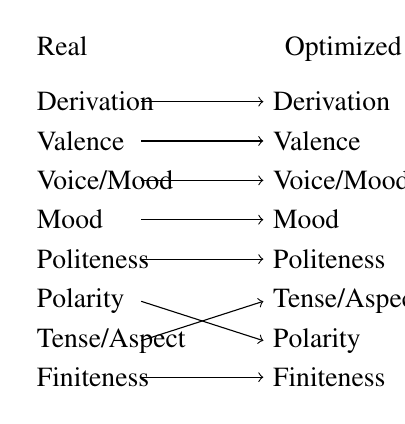
\begin{tikzpicture}[%
% common options for blocks:
block/.style = {draw, fill=blue!30, align=center, anchor=west,
            minimum height=0.65cm, inner sep=0},
% common options for the circles:
ball/.style = {circle, draw, align=center, anchor=north, inner sep=0}]
\node[rectangle,text width=1.2cm,anchor=base] (A0) at (1,-0.3) {Real};
\node[rectangle,text width=0.9cm,anchor=base] (B0) at (4,-0.3) {Optimized};
\node[rectangle,text width=1.2cm,anchor=base] (A1) at (1,-1.0) {Derivation};
\node[rectangle,text width=1.2cm,anchor=base] (A2) at (1,-1.5) {Valence};
\node[rectangle,text width=1.2cm,anchor=base] (A3) at (1,-2.0) {Voice/Mood};
\node[rectangle,text width=1.2cm,anchor=base] (A4) at (1,-2.5) {Mood};
\node[rectangle,text width=1.2cm,anchor=base] (A5) at (1,-3.0) {Politeness};
\node[rectangle,text width=1.2cm,anchor=base] (A6) at (1,-3.5) {Polarity};
\node[rectangle,text width=1.2cm,anchor=base] (A7) at (1,-4.0) {Tense/Aspect};
\node[rectangle,text width=1.2cm,anchor=base] (A8) at (1,-4.5) {Finiteness};
\node[rectangle,text width=1.2cm,anchor=base] (B1) at (4,-1.0) {Derivation};
\node[rectangle,text width=1.2cm,anchor=base] (B2) at (4,-1.5) {Valence};
\node[rectangle,text width=1.2cm,anchor=base] (B3) at (4,-2.0) {Voice/Mood};
\node[rectangle,text width=1.2cm,anchor=base] (B4) at (4,-2.5) {Mood};
\node[rectangle,text width=1.2cm,anchor=base] (B5) at (4,-3.0) {Politeness};
\node[rectangle,text width=1.2cm,anchor=base] (B6) at (4,-3.5) {Tense/Aspect};
\node[rectangle,text width=1.2cm,anchor=base] (B7) at (4,-4.0) {Polarity};
\node[rectangle,text width=1.2cm,anchor=base] (B8) at (4,-4.5) {Finiteness};
\draw[->] (A1.east) to (B1.west);
\draw[->] (A2.east) to (B2.west);
\draw[->] (A3.east) to (B3.west);
\draw[->] (A4.east) to (B4.west);
\draw[->] (A5.east) to (B5.west);
\draw[->] (A6.east) to (B7.west);
\draw[->] (A7.east) to (B6.west);
\draw[->] (A8.east) to (B8.west);
\end{tikzpicture}

  \end{minipage}
  &
  \begin{minipage}{.3\textwidth}
    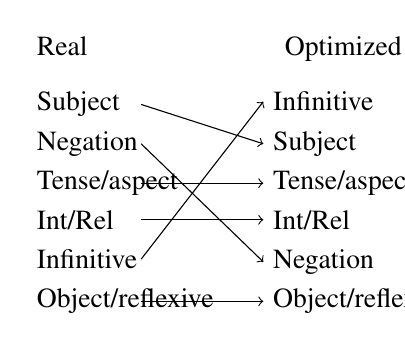
\begin{tikzpicture}[%
% common options for blocks:
block/.style = {draw, fill=blue!30, align=center, anchor=west,
            minimum height=0.65cm, inner sep=0},
% common options for the circles:
ball/.style = {circle, draw, align=center, anchor=north, inner sep=0}]
\node[rectangle,text width=1.2cm,anchor=base] (A0) at (1,-0.3) {Real};
\node[rectangle,text width=0.9cm,anchor=base] (B0) at (4,-0.3) {Optimized};
\node[rectangle,text width=1.2cm,anchor=base] (A1) at (1,-1.0) {Subject};
\node[rectangle,text width=1.2cm,anchor=base] (A2) at (1,-1.5) {Negation};
\node[rectangle,text width=1.2cm,anchor=base] (A3) at (1,-2.0) {Tense/aspect};
\node[rectangle,text width=1.2cm,anchor=base] (A4) at (1,-2.5) {Int/Rel};
\node[rectangle,text width=1.2cm,anchor=base] (A5) at (1,-3.0) {Infinitive};
\node[rectangle,text width=1.2cm,anchor=base] (A6) at (1,-3.5) {Object/reflexive};
\node[rectangle,text width=1.2cm,anchor=base] (B1) at (4,-1.0) {Infinitive};
\node[rectangle,text width=1.2cm,anchor=base] (B2) at (4,-1.5) {Subject};
\node[rectangle,text width=1.2cm,anchor=base] (B3) at (4,-2.0) {Tense/aspect};
\node[rectangle,text width=1.2cm,anchor=base] (B4) at (4,-2.5) {Int/Rel};
\node[rectangle,text width=1.2cm,anchor=base] (B5) at (4,-3.0) {Negation};
\node[rectangle,text width=1.2cm,anchor=base] (B6) at (4,-3.5) {Object/reflexive};
\draw[->] (A1.east) to (B2.west);
\draw[->] (A2.east) to (B5.west);
\draw[->] (A3.east) to (B3.west);
\draw[->] (A4.east) to (B4.west);
\draw[->] (A5.east) to (B1.west);
\draw[->] (A6.east) to (B6.west);
\end{tikzpicture}

  \end{minipage} \\
  \textsc{Sesotho Suffixes} \\
  \begin{minipage}{.3\textwidth}
    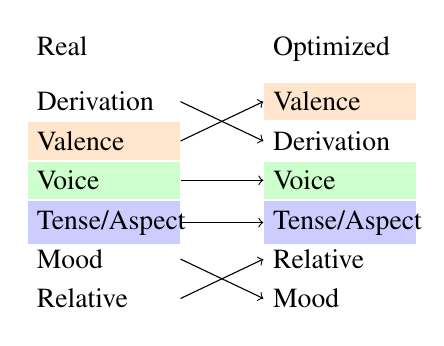
\begin{tikzpicture}[%
% common options for blocks:
block/.style = {draw, fill=blue!30, align=center, anchor=west,
            minimum height=0.65cm, inner sep=0},
% common options for the circles:
ball/.style = {circle, draw, align=center, anchor=north, inner sep=0}]
\node[rectangle,text width=1.7cm,anchor=base] (A0) at (1,-0.3) {Real};
\node[rectangle,text width=1.7cm,anchor=base] (B0) at (4,-0.3) {Optimized};
\node[rectangle,text width=1.7cm,anchor=base] (A1) at (1,-1.0) {Derivation};
\node[rectangle,text width=1.7cm,anchor=base, fill=orange!20] (A2) at (1,-1.5) {Valence};
\node[rectangle,text width=1.7cm,anchor=base, fill=green!20] (A3) at (1,-2.0) {Voice};
\node[rectangle,text width=1.7cm,anchor=base, fill=blue!20] (A4) at (1,-2.5) {Tense/Aspect};
\node[rectangle,text width=1.7cm,anchor=base] (A5) at (1,-3.0) {Mood};
\node[rectangle,text width=1.7cm,anchor=base] (A6) at (1,-3.5) {Relative};
\node[rectangle,text width=1.7cm,anchor=base, fill=orange!20] (B1) at (4,-1.0) {Valence};
\node[rectangle,text width=1.7cm,anchor=base] (B2) at (4,-1.5) {Derivation};
\node[rectangle,text width=1.7cm,anchor=base, fill=green!20] (B3) at (4,-2.0) {Voice};
\node[rectangle,text width=1.7cm,anchor=base, fill=blue!20] (B4) at (4,-2.5) {Tense/Aspect};
\node[rectangle,text width=1.7cm,anchor=base] (B5) at (4,-3.0) {Relative};
\node[rectangle,text width=1.7cm,anchor=base] (B6) at (4,-3.5) {Mood};
\draw[->] (A1.east) to (B2.west);
\draw[->] (A2.east) to (B1.west);
\draw[->] (A3.east) to (B3.west);
\draw[->] (A4.east) to (B4.west);
\draw[->] (A5.east) to (B6.west);
\draw[->] (A6.east) to (B5.west);
\end{tikzpicture}

  \end{minipage}
  \end{tabular}
  
  
    \caption{Real and optimized ordering for verb affixes. Colors indicate universal position slots as in Figure~\ref{tab:examples-verbs}.
    \mhahn{figure out how to make size of boxes large enough for text to fit in}%\mhahn{TODO make sure the language-specific morpheme slots such as ``Genitive'' and ``Clitic'' aren't confusing for the reader. One option is to color-code the slots here as in the figure(s) earlier.}
    \mhahn{TODO make this look nicer}
    }
    \label{fig:real_and_optimized_verbs}
\end{figure}




\section{Discussion}\label{sec:discussion}



We have examined morpheme order in nouns and verbs in six morphologically rich agglutinating languages, testing the recently proposed Efficient Tradeoff Hypothesis \citep{Hahn2020modeling} as an explanatory account of morpheme ordering.
We compared actual morpheme orderings to other possible orderings and to orderings optimized for efficiency of the memory-surprisal tradeoff.
In most cases, we found that the real ordering provided more efficient tradeoffs than most alternative orderings.
More importantly, we found that the real orderings match the optimal orderings with high accuracy.
%Ordering forms found in a corpus according to real or optimized orderings yields the same orders in the large majority of cases. \becky{A little hard to understand -- maybe just delete this previous sentence?}
In some cases, particularly for noun inflection, the match between real and optimized orderings is perfect.
Beyond language-specific ordering patterns, optimization recovers previously-documented language universals of morpheme order.
These results support the idea that optimization for processing effort can explain universals of morpheme ordering.





\subsection{Limitations}

%- limitations of computational estimation of the memory-surprisal tradeoff. %However: As the set of all moprphological forms of a language is typically finite (CITE), we believe that these limitations play a smaller role in morpheme order, compared to word order.

A limitation of this study is that memory-surprisal tradeoffs are estimated on finite datasets that do not cover all possible morphological forms of a language. However, to the extent that this limitation impacts the estimation of memory-surprisal tradeoffs, it should equally apply to real and counterfactual orderings. We thus do not expect the relative measured efficiencies of different orderings to be impacted by the finiteness of data.

Due to limitations in data availability, this study builds on languages from Eurasia and Africa, not representing Australia and America.
Among the languages, Hungarian and Finnish are genetically related, sharing a common ancestor about 5,000 years ago \citep{maurits2020best}.
There is also some evidence for genetic relations beyond these (Japanese, Korean, Turkish), but such relations would have to be quite ancient.
Importantly, the morphemes found in these languages as considered here are generally not cognate.
Thus, the commonalities across languages found cannot be traced to inherited orderings of morphemes that are inherited from a common ancestor.
%Furthermore, we note that the predictions of the Efficient Tradeoff Hypothesis of different orderings crucially depend not on the morphemes themselves (which might be inherited), but on the usage frequencies of different forms (e.g., of singulars and plurals).


%- genre of data: written. but Sesotho is spoken (child-directed)
%A further limitation relates to the selection of languages.
%The six languages considered in this study are spoken in Eurasia and Africa, not representing Australia and America.


\subsection{Relation to previous accounts}


In this section, we relate our results to existing explanatory accounts of morpheme ordering reviewed in Section~\ref{sec:previous}.
In a review of research on morpheme ordering, \citet{manova2010modeling} % https://homepage.univie.ac.at/stela.manova/modeling%20affix%20order.pdf
categorize approaches to morpheme ordering into three classes (similarly \citet{rice2000morpheme, rice2011principles}): orderings that are motivated by properties of syntax, semantics or phonology (\textit{grammatical theories}); orderings that are motivated by human language processing responding to statistical properties of language (\textit{processing theories}); and orderings that are arbitrarily stipulated  (\textit{arbitrary orderings}).
Our approach falls into the second class, explaining morpheme ordering based on minimization of human processing effort.
In this section, we describe how our account relates to other accounts across these three clusters, and show how the memory-surprisal tradeoff has tight connections with notions proposed across seemingly very different accounts.

%\mhahn{One can debate whether this trichotony is right -- e.g. Bybee's approach could be thought of as cognitive. What the second class 


%- citing \cite{rice2000morpheme}; Manova and Aronoff 2010; Saarinen and Hay 2014
%Rice states three types of explanations/phenomena:
%- extra-grammatical: frequency, productivity, parsability


\paragraph{Relation to Grammatical Theories}

\citet{bybee-morphology-1985} argues that morphemes that are semantically more relevant to the root are ordered closer to it.
We suggest that mutual information provides an operational formalization of semantic relevance.
For instance, according to Bybee, passive markers are more relevant to the root than TAM markers, as they alter the verb's argument structure.
We also expect that they have high mutual information with the verb stem, since only certain verbs (typically a subclass of the transitive verbs) can form a passive.
The idea that mutual information is an operationalization of semantic closeness has also been suggested in other places; for instance, \citet{culbertson2020from} link mutual information to conceptual closeness as a driving factor of noun phrase modification.


\mhahn{there is also the following commented-out section. these arguments are a bit speculative and not fleshed out. I feel like if we want to make those arguments, we might need to refer to SI sections where we go into a bit more detail, to avoid crowding the Discussion with relatively specialized discussion. What do you think?}

%A similar argument can be made for the scope-based account, which holds that morphemes are ordered in the order in which their meanings combine to form the meaning of the full word \citep{rice2000morpheme}.
%However, there are arguments that scope relations correlate with mutual information.
%\citet{culbertson2020from} made a related argument for the order of nominal modifiers as in ``the four green books'', where mutual information predicts the order of attachment of modifiers to the noun.
%Furthermore, if the semantic propositions that speakers communicate are modeled using a probabilistic language-of-thought grammar such as mutual information will also correlate with scope ordering (see SI Appendix Section S4 for a simulation study).




Other grammatical accounts explain morpheme order in terms of a parallelism to word order, either through diachronic fossilization of words into affixes or through synchronic constraints on language \citep{givon1971historical,venneman1973explanation,baker1985the}.
As a theory of order at multiple levels, the Efficient Tradeoff Hypothesis is compatible with parallelism between morpheme and word order.
%\mhahn{TODO maybe say nore here}


\paragraph{Relation to Previous Processing Accounts}

The theory of Complexity-Based Ordering \citep{hay2002speech,plag2002the,hay2004what,hay2005shifting,plag2009suffix}.
holds that affixes are closer to the root when they are less ``separable'', where separability indicates the productivity of an affix and the likelihood that affixes are processed separately with the base in human lexical access  \citep{baayen1993on}.
%In particular, affixes are less ``separable'' when they are processed holistically together with the base in human lexical access \citep{baayen1993on}. %, such as in the dual processing race model of morphological access, which asserts that morphological forms can be processed either separately in terms of its components or as a whole \citep{baayen1993on}.
%Forms are more separable if they are less likely to be processed together with the root (Baayen \& Schreuder 1999, Baayen \& Moscoso del Prado Mart ́ın 2005).
%also mention \cite{manova2010suffix}
%\cite{plag2009suffix} %http://www.sfs.uni-tuebingen.de/~hbaayen/publications/plagBaayenLanguage2009.pdf
A statistical operationalization of separability is in terms of relative frequencies:
affixes are more likely to be processed together with the root when the composite form has a higher frequency compared to the base form \citep{hay2001lexical}. % , lee2011ordering
This has an interesting relation to mutual information: 
If the compound form is very frequent, in relation to the baseline frequencies of the base and the affix, then there is high (pointwise) mutual information between them.
%\mhahn{Make clear that this theory hasn't been applied to the kinds of affix orderin generalizations that we look at in this paper.}

\mhahn{I'm pondering whether it would be beneficial to do some more explicit comparison using actual formulas both complexity-based ordering and perhaps the Inkelas 2016 idea, either here or in an SI section (the advantage of the latter would be that explanations can be more thorough without dominating the Discussion section) let me know what you think!}

The Efficient Tradeoff Hypothesis is also related to the proposal of \citet{inkelas2016affix} that morphemes are ordered together when they are informative about each other.
While their notion of informativity \citep{priva2017informativity} is different from mutual information, the two quantities are related (see SI Appendix Section X for details).
%Formally (drawing on the notion of informativity defined by \citet{priva2017informativity}), they considered the informativity between a suffix $S_i$ and the preceding $S_{i-1}$ as 
%\begin{equation}
%    \sum_{S_{i-1}, S_{i}} \frac{P(S_{i-1} , S_i)}{P(S_i)} \log P(S_i | S_{i-1})
%\end{equation}
%They tested this idea in a pilot study of Turkish, finding preliminary evidence that high-informativity suffixes are closer to the root.
%This notion of informativity is similar to $I_1$, only differing in whether the $P(S_i)$ term occurs inside the logarithm:
%\begin{equation}
%   I_1 = \sum_{S_{i-1}, S_{i}} P(S_{i-1} , S_i) \log \frac{P(S_i | S_{i-1})}{P(S_i)}
%\end{equation}


%Inkelas: informativity: they propose that bigram surprisal is minimized (not their terminology), test this in a pilot study of Turkish, with partially confirming results \citep{inkelas2015informativity}
%Alternatively, the lower thefrequency of the derived word in relation to the base word, the more important the role ofthe constituents become
%Hay and Plag (2004) show that ordering correlates with relative frequency and productivity
%Hay (in press) distinguishes between derived forms which are more frequent than the bases they contain (e.g.illegible is more frequent than legible), and derived forms whic hare less frequent than their bases (e.g.illiberal is less frequent than liberal).
% argues that whether an affix is processed together with the root is determined in part by the relative frequency
%\begin{equation}
%    \frac{P(base+affix)}{P(base)}
%\end{equation}
%\begin{equation}
%    \log \frac{P(base, affix)}{P(base)} = \log P(affix|base)
%\end{equation}
%\begin{equation}
%    pmi(base, affix) = \log \frac{p(affix|base)}{p(base)}
%\end{equation}
%Hay and Baayen (2002).
%Hay and Plag (2004): parsing ratio and productivity measured by Hay and Baayen (2002).
%Complexity-based Ordering, the position of a given suffix inthe hierarchy reflects the degree to which that suffix is processed independently of its base.

%\citet{hay2004what} propose a model of complexity-based ordering based on processing considerations, called complexity-based ordering, arguing that affixes are further away from the root when they can be separated more easily in processing, testing this theory using 15 English affixes.


%from Inkelas



\paragraph{Relations to Accounts Stipulating Arbitrary Orderings}

There are also studies suggesting language-specific and essentially arbitrary properties of morpheme ordering.
A classical approach to describing morpheme ordering is in terms of levels, where morphemes from a higher level occur before morphemes from a lower level \citep{siegel1979topics}, and in terms of templates that describe the ordering of morphemes \citep{simpson1986pronominal,spencer1991morphological,stump1992on,inkelas1993nimboran,hyman2003suffix,nordlinger2010verbal}.
Ordering based on language-specific templates has been proposed specifically in cases where observed morpheme ordering is in conflict with semantic scope, as in Bantu languages \citep{hyman2003suffix}.
\citet{fabb1988english} prominently describes English affix ordering in terms of the selectional restrictions that individual affixes place on which other affixes they can attach to.
While this approach does not make statements as to which affixes would go closer to the base in a given language, it does suggest that morpheme ordering is described based on the pairwise interactions between adjacent morphemes.
In a similar vein, \citet{ryan2010variable} propose a model based on weighted bigram constraints in Tagalog, for the (rather uncommon) case of flexible morpheme ordering.
Ordering constraints operating on adjacent pairs of morphemes might provide relatively efficient memory-surprisal tradeoffs because the appearance of a morpheme is constrained only by its immediately adjacent morphemes.




%Tension between Scope and templatic: \citep{hyman2003suffix}; \cite{aronoff2010introduction}; \cite{spencer2003putting}
%- arbitrary language-specific tenplatic (Fabb 1988 English affix ordering; position class templates, Simpson and Withgott 1986) (also finite-state automata Hankamer 1986; Karttunen 2003) 

%re scope also \cite{alsina1999where}

%\cite{manova2010modeling} % https://homepage.univie.ac.at/stela.manova/modeling%20affix%20order.pdf
%also provide a ctagoeirzation into grammatical, psycholinguistic, unmotivated (among others)





%\cite{aronoff2010a} % Within this model, phonological form is spelled out by means of individual-language-particular realization constraints that associate abstract morphosyntactic feature values with phonological forms and that are ordered among more general constraints governing factors like scope and feature splitting. The data used to exemplify the application of our theory to affix order are drawn from Haspelmath’s (A grammar of Lezgian, Mouton de Gruyter, Berlin, 1993) grammar of Lezgian, a language of the Northeast Caucasian family spoken largely in Dagestan (Russia) and Azerbaijan.



%\paragraph{Templates}
%CARP template
%\cite{muysken1981quechua}
%\cite{mccarthy2008generalized} phonology
%\cite{hyman2003suffix}
%\cite{kanu2009suffix} morphotactics, not semantic scope



\subsection{Other Aspects of Morphology}

Our study focused on agglutination, where a word carries multiple clearly separated morphemes with distinct functions.
There are other types of morphological processes that deserve study.
Many languages show fusion \citep{wals-20} where different categories are fused into a single morpheme, or stem changes, such as English \textit{swim} $\rightarrow$ \textit{swam}.
An extreme case is non-concatenative morphology (e.g., in Arabic, k-t-b `to write' forms \textit{katab}- `wrote'. -\textit{aktub} `write/be writing', -\textit{kutib}- `was written').
These types of morphological processes are not described in terms of the order of different morphemes.
We leave it to future research to determine whether these processes are also constrained by cognitive considerations of processing efficiency.

While we have focused on the relative distance from the root, we have not touched on the question of why a morpheme is realized as a prefix or a suffix in a given language.
There are well-known correlations between suffixing or prefixing preference and word order \citep{greenberg1963universals}.
It is an interesting problem for future research to study whether these correlations might arise from processing efficiency optimization.




\section{Conclusion}

We have tested the recently proposed Efficient Tradeoff Hypothesis as a predictor of morpheme order with data from verbs and nouns across six languages.
We found that attested morpheme orders provide more efficient tradeoffs than most other possible orderings and that many properties of observed orderings are recovered by optimizing for tradeoff efficiency.
With the exception of verb inflection in Finnish and Sesotho, we found that optimized orderings agree with the attested orderings in more than 90\% of forms found in corpora.
Optimization also successfully predicts several universals of morpheme ordering, both for nouns and verbs.
These results suggest that morpheme ordering reflects optimization of processing efficiency across languages.
%\jd{add concluding sentence tying all together}


\printbibliography

\end{document}




\begin{figure}

  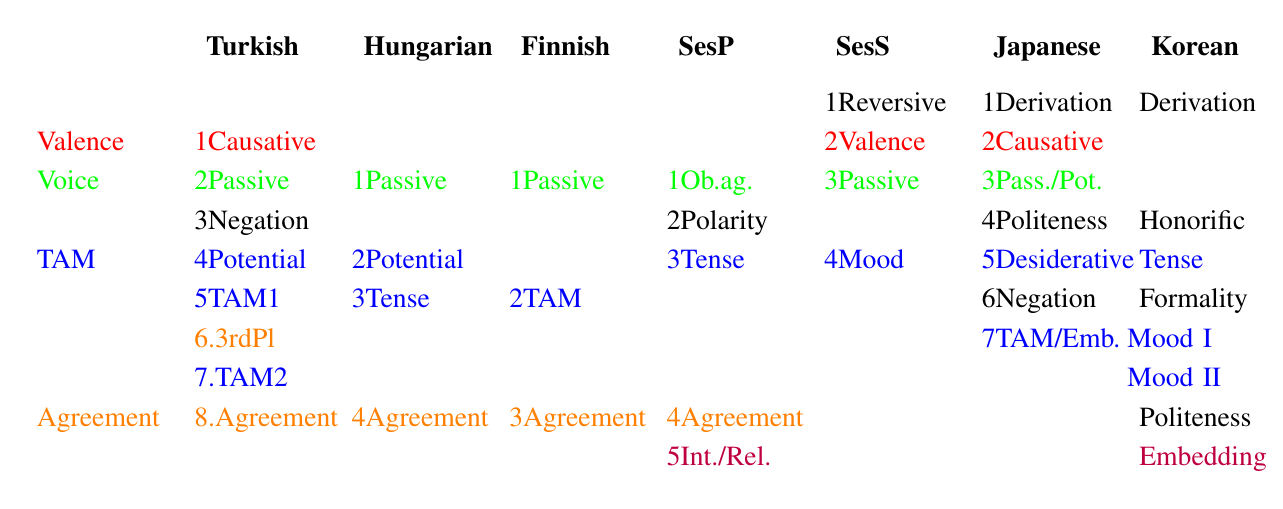
\begin{tikzpicture}[%
% common options for blocks:
block/.style = {draw, fill=blue!30, align=center, anchor=west,
            minimum height=0.65cm, inner sep=0},
% common options for the circles:
ball/.style = {circle, draw, align=center, anchor=north, inner sep=0}]
%\node[rectangle,text width=1.2cm,anchor=base] (A0) at (1,-0.3) {Real};

%\node[rectangle,text width=5cm,anchor=left, color=red, fill=red, opacity=0.1] (A02) at (1,-1.5) {};

%\node[rectangle,text width=1.2cm,anchor=base] (A1) at (1,-1.0) {1Derivation};
\node[rectangle,text width=1.2cm,anchor=base, color=red] (A2) at (1,-1.5) {Valence};
\node[rectangle,text width=1.2cm,anchor=base, color=green] (A3) at (1,-2.0) {Voice};
\node[rectangle,text width=1.2cm,anchor=base,color=blue] (A4) at (1,-3) {TAM};
%\node[rectangle,text width=1.2cm,anchor=base,color=blue] (A4) at (1,-3.5) {Tense};
%\node[rectangle,text width=1.2cm,anchor=base,color=blue] (A4) at (1,-4) {Mood};
\node[rectangle,text width=1.2cm,anchor=base,color=orange] (A4) at (1,-5) {Agreement};

% Turkish
\node[rectangle,text width=0.9cm,anchor=base] (B0) at (3,-0.3) {\textbf{Turkish}};
\node[rectangle,text width=1.2cm,anchor=base,color=red] (B1) at (3,-1.5) {1Causative};
\node[rectangle,text width=1.2cm,anchor=base,color=green] (B2) at (3,-2) {2Passive};
\node[rectangle,text width=1.2cm,anchor=base] (B3) at (3,-2.5) {3Negation};
\node[rectangle,text width=1.2cm,anchor=base,color=blue] (B4) at (3,-3) {4Potential};
\node[rectangle,text width=1.2cm,anchor=base,color=blue] (B4) at (3,-3.5) {5TAM1};
\node[rectangle,text width=1.2cm,anchor=base,color=orange] (B4) at (3,-4) {6.3rdPl};
\node[rectangle,text width=1.2cm,anchor=base,color=blue] (B4) at (3,-4.5) {7.TAM2};
\node[rectangle,text width=1.2cm,anchor=base,color=orange] (B4) at (3,-5) {8.Agreement};

% Hungarian
\node[rectangle,text width=0.9cm,anchor=base] (B0) at (5,-0.3) {\textbf{Hungarian}};
\node[rectangle,text width=1.2cm,anchor=base,color=green] (B2) at (5,-2) {1Passive};
\node[rectangle,text width=1.2cm,anchor=base,color=blue] (B4) at (5,-3) {2Potential};
\node[rectangle,text width=1.2cm,anchor=base,color=blue] (B4) at (5,-3.5) {3Tense};
\node[rectangle,text width=1.2cm,anchor=base,color=orange] (B4) at (5,-5) {4Agreement};


% Finnish
\node[rectangle,text width=0.9cm,anchor=base] (B0) at (7,-0.3) {\textbf{Finnish}};
\node[rectangle,text width=1.2cm,anchor=base,color=green] (B2) at (7,-2) {1Passive};
\node[rectangle,text width=1.2cm,anchor=base,color=blue] (B4) at (7,-3.5) {2TAM};
\node[rectangle,text width=1.2cm,anchor=base,color=orange] (B4) at (7,-5) {3Agreement};

% Sesotho Prefixes
\node[rectangle,text width=0.9cm,anchor=base] (B0) at (9,-0.3) {\textbf{SesP}};
\node[rectangle,text width=1.2cm,anchor=base,color=green] (B2) at (9,-2) {1Ob.ag.};
\node[rectangle,text width=1.2cm,anchor=base] (B4) at (9,-2.5) {2Polarity};
\node[rectangle,text width=1.2cm,anchor=base,color=blue] (B4) at (9,-3) {3Tense};
\node[rectangle,text width=1.2cm,anchor=base,color=orange] (B4) at (9,-5) {4Agreement};
\node[rectangle,text width=1.2cm,anchor=base,color=purple] (B4) at (9,-5.5) {5Int./Rel.};

% Sesotho Suffixes
\node[rectangle,text width=0.9cm,anchor=base] (B0) at (11,-0.3) {\textbf{SesS}};
\node[rectangle,text width=1.2cm,anchor=base] (B2) at (11,-1) {1Reversive};
\node[rectangle,text width=1.2cm,anchor=base,color=red] (B2) at (11,-1.5) {2Valence};
\node[rectangle,text width=1.2cm,anchor=base,color=green] (B2) at (11,-2) {3Passive};
\node[rectangle,text width=1.2cm,anchor=base,color=blue] (B4) at (11,-3) {4Mood};



% Japanese
\node[rectangle,text width=0.9cm,anchor=base] (B0) at (13,-0.3) {\textbf{Japanese}};
\node[rectangle,text width=1.2cm,anchor=base] (B2) at (13,-1) {1Derivation};
\node[rectangle,text width=1.2cm,anchor=base,color=red] (B2) at (13,-1.5) {2Causative};
\node[rectangle,text width=1.2cm,anchor=base,color=green] (B2) at (13,-2) {3Pass./Pot.};
\node[rectangle,text width=1.2cm,anchor=base] (B4) at (13,-2.5) {4Politeness};
\node[rectangle,text width=1.2cm,anchor=base,color=blue] (B4) at (13,-3) {5Desiderative};
\node[rectangle,text width=1.2cm,anchor=base] (B4) at (13,-3.5) {6Negation};
\node[rectangle,text width=1.2cm,anchor=base,color=blue] (B4) at (13,-4) {7TAM/Emb.};

% Korean
\node[rectangle,text width=0.9cm,anchor=base] (B0) at (15,-0.3) {\textbf{Korean}};
\node[rectangle,text width=1.2cm,anchor=base] (B2) at (15,-1.0) {Derivation};
\node[rectangle,text width=1.2cm,anchor=base] (B4) at (15,-2.5) {Honorific};
\node[rectangle,text width=1.2cm,anchor=base,color=blue] (B4) at (15,-3) {Tense};
\node[rectangle,text width=1.2cm,anchor=base] (B4) at (15,-3.5) {Formality};
\node[rectangle,text width=1.5cm,anchor=base,color=blue] (B4) at (15,-4.0) {Mood I};
\node[rectangle,text width=1.5cm,anchor=base,color=blue] (B4) at (15,-4.5) {Mood II};
\node[rectangle,text width=1.2cm,anchor=base] (B4) at (15,-5) {Politeness};
\node[rectangle,text width=1.2cm,anchor=base,color=purple] (B4) at (15,-5.5) {Embedding};


%\draw[->] (A1.east) to (B1.west);
%\draw[->] (A2.east) to (B2.west);
%\draw[->] (A3.east) to (B3.west);
%\draw[->] (A4.east) to (B4.west);
\end{tikzpicture}

%    \centering
%\begin{tabular}{l||l|l|l|l|l|l|llll}
%                    & Turkish & Hungarian & Finnish  & Sesotho Pref.     & Ses Suff. & Japanese & Korean\\ \hline\hline
%Derivation          &  &         &          &               & Reversive & suru    & ha,i\\ \hline
%Valence             &  Causative &         &           & Object marker & Valence & Causative\\ \hline
%Voice               & Passive & Passive    & Passive     &               & Passive & Passive\\ \hline
%TAM, Pol.           & Negation  &   Potential  &   Tense/Asp &    Negation &  Politeness &      Potential        & Honorific \\
%                    & Potential & Tense        &    Mood     &     Tense   &    Mood     &   Honorific  &    Tense       \\
%                    &   TAM1    &          &                &         &                  & Tense/Aspect & Formality \\
%                    & lar       &          &           &  & & Negation & Mood I\\
%                    & TAM2         &           &               &          &       &      &  Mood II \\ \hline
%Agreement           & Agreement & Agreement & Agreement & Agreement \\ \hline
%\textit{Other}               & Formality          & Clitic    &              & Int/Rel &      &        & Politeness \\
%                    &           &     &              &  &          &    & Conj \\
%\end{tabular}

\mhahn{TODO make this visually more appealing}

    \caption{Morpheme order across the six languages in our sample, matched with four universal categories (left).}
    \label{tab:examples-verbs}
\end{figure}




\begin{figure}
\begin{tabular}{ccccccc}
\textsc{Finnish} & \textsc{Hungarian} & \textsc{Turkish} \\
\begin{minipage}{.3\textwidth}
    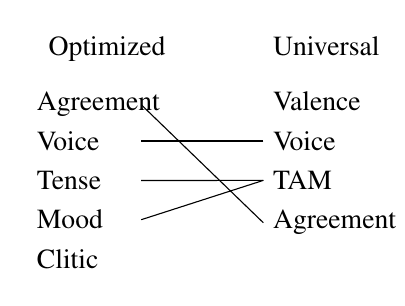
\begin{tikzpicture}[%
% common options for blocks:
block/.style = {draw, fill=blue!30, align=center, anchor=west,
            minimum height=0.65cm, inner sep=0},
% common options for the circles:
ball/.style = {circle, draw, align=center, anchor=north, inner sep=0}]
\node[rectangle,text width=1.2cm,anchor=base] (A0) at (4,-0.3) {Universal};
\node[rectangle,text width=0.9cm,anchor=base] (B0) at (1,-0.3) {Optimized};
\node[rectangle,text width=1.2cm,anchor=base] (A1) at (4,-1.0) {Valence};
\node[rectangle,text width=1.2cm,anchor=base] (A2) at (4,-1.5) {Voice};
\node[rectangle,text width=1.2cm,anchor=base] (A3) at (4,-2.0) {TAM};
\node[rectangle,text width=1.2cm,anchor=base] (A4) at (4,-2.5) {Agreement};
\node[rectangle,text width=1.2cm,anchor=base] (B1) at (1,-1.0) {Agreement};
\node[rectangle,text width=1.2cm,anchor=base] (B2) at (1,-1.5) {Voice};
\node[rectangle,text width=1.2cm,anchor=base] (B3) at (1,-2.0) {Tense};
\node[rectangle,text width=1.2cm,anchor=base] (B4) at (1,-2.5) {Mood};
\node[rectangle,text width=1.2cm,anchor=base] (B5) at (1,-3.0) {Clitic};
\draw[-] (A4.west) to (B1.east);
\draw[-] (A2.west) to (B2.east);
\draw[-] (A3.west) to (B3.east);
\draw[-] (A3.west) to (B4.east);
\end{tikzpicture}

    \end{minipage}
    &
    \begin{minipage}{.3\textwidth}
    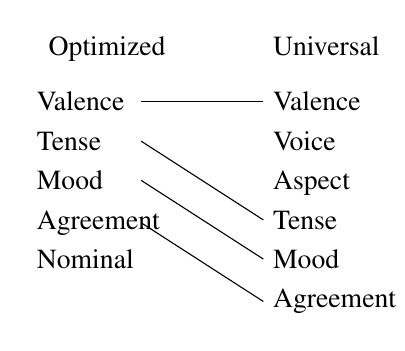
\begin{tikzpicture}[%
% common options for blocks:
block/.style = {draw, fill=blue!30, align=center, anchor=west,
            minimum height=0.65cm, inner sep=0},
% common options for the circles:
ball/.style = {circle, draw, align=center, anchor=north, inner sep=0}]
\node[rectangle,text width=1.2cm,anchor=base] (A0) at (4,-0.3) {Universal};
\node[rectangle,text width=0.9cm,anchor=base] (B0) at (1,-0.3) {Optimized};
\node[rectangle,text width=1.2cm,anchor=base] (A1) at (4,-1.0) {Valence};
\node[rectangle,text width=1.2cm,anchor=base] (A2) at (4,-1.5) {Voice};
\node[rectangle,text width=1.2cm,anchor=base] (A3) at (4,-2.0) {Aspect};
\node[rectangle,text width=1.2cm,anchor=base] (A4) at (4,-2.5) {Tense};
\node[rectangle,text width=1.2cm,anchor=base] (A5) at (4,-3.0) {Mood};
\node[rectangle,text width=1.2cm,anchor=base] (A6) at (4,-3.5) {Agreement};
\node[rectangle,text width=1.2cm,anchor=base] (B1) at (1,-1.0) {Valence};
\node[rectangle,text width=1.2cm,anchor=base] (B2) at (1,-1.5) {Tense};
\node[rectangle,text width=1.2cm,anchor=base] (B3) at (1,-2.0) {Mood};
\node[rectangle,text width=1.2cm,anchor=base] (B4) at (1,-2.5) {Agreement};
\node[rectangle,text width=1.2cm,anchor=base] (B5) at (1,-3.0) {Nominal};
\draw[-] (A1.west) to (B1.east);
\draw[-] (A4.west) to (B2.east);
\draw[-] (A5.west) to (B3.east);
\draw[-] (A6.west) to (B4.east);
\end{tikzpicture}

    \end{minipage}
        &
    \begin{minipage}{.3\textwidth}
    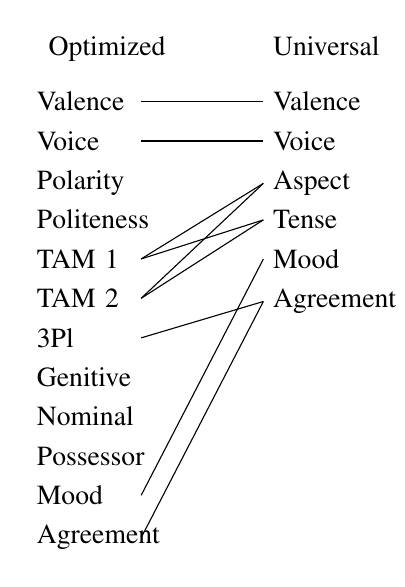
\begin{tikzpicture}[%
% common options for blocks:
block/.style = {draw, fill=blue!30, align=center, anchor=west,
            minimum height=0.65cm, inner sep=0},
% common options for the circles:
ball/.style = {circle, draw, align=center, anchor=north, inner sep=0}]
\node[rectangle,text width=1.2cm,anchor=base] (A0) at (4,-0.3) {Universal};
\node[rectangle,text width=0.9cm,anchor=base] (B0) at (1,-0.3) {Optimized};
\node[rectangle,text width=1.2cm,anchor=base] (A1) at (4,-1.0) {Valence};
\node[rectangle,text width=1.2cm,anchor=base] (A2) at (4,-1.5) {Voice};
\node[rectangle,text width=1.2cm,anchor=base] (A3) at (4,-2.0) {Aspect};
\node[rectangle,text width=1.2cm,anchor=base] (A4) at (4,-2.5) {Tense};
\node[rectangle,text width=1.2cm,anchor=base] (A5) at (4,-3.0) {Mood};
\node[rectangle,text width=1.2cm,anchor=base] (A6) at (4,-3.5) {Agreement};
\node[rectangle,text width=1.2cm,anchor=base] (B1) at (1,-1.0) {Valence};
\node[rectangle,text width=1.2cm,anchor=base] (B2) at (1,-1.5) {Voice};
\node[rectangle,text width=1.2cm,anchor=base] (B3) at (1,-2.0) {Polarity};
\node[rectangle,text width=1.2cm,anchor=base] (B4) at (1,-2.5) {Politeness};
\node[rectangle,text width=1.2cm,anchor=base] (B5) at (1,-3.0) {TAM 1};
\node[rectangle,text width=1.2cm,anchor=base] (B6) at (1,-3.5) {TAM 2};
\node[rectangle,text width=1.2cm,anchor=base] (B7) at (1,-4.0) {3Pl};
\node[rectangle,text width=1.2cm,anchor=base] (B8) at (1,-4.5) {Genitive};
\node[rectangle,text width=1.2cm,anchor=base] (B9) at (1,-5.0) {Nominal};
\node[rectangle,text width=1.2cm,anchor=base] (B10) at (1,-5.5) {Possessor};
\node[rectangle,text width=1.2cm,anchor=base] (B11) at (1,-6.0) {Mood};
\node[rectangle,text width=1.2cm,anchor=base] (B12) at (1,-6.5) {Agreement};
\draw[-] (A1.west) to (B1.east);
\draw[-] (A2.west) to (B2.east);
\draw[-] (A3.west) to (B5.east);
\draw[-] (A4.west) to (B5.east);
\draw[-] (A3.west) to (B6.east);
\draw[-] (A4.west) to (B6.east);
\draw[-] (A6.west) to (B7.east);
\draw[-] (A5.west) to (B11.east);
\draw[-] (A6.west) to (B12.east);
\end{tikzpicture}

    \end{minipage} 
    \\
    \textsc{Korean} & \textsc{Japanese} & \textsc{Sesotho Prefixes} \\
        \begin{minipage}{.3\textwidth}
    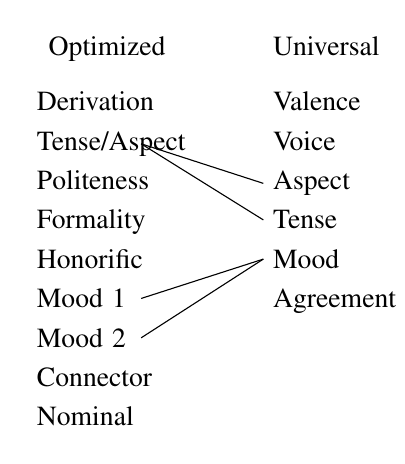
\begin{tikzpicture}[%
% common options for blocks:
block/.style = {draw, fill=blue!30, align=center, anchor=west,
            minimum height=0.65cm, inner sep=0},
% common options for the circles:
ball/.style = {circle, draw, align=center, anchor=north, inner sep=0}]
\node[rectangle,text width=1.2cm,anchor=base] (A0) at (4,-0.3) {Universal};
\node[rectangle,text width=0.9cm,anchor=base] (B0) at (1,-0.3) {Optimized};
\node[rectangle,text width=1.2cm,anchor=base] (A1) at (4,-1.0) {Valence};
\node[rectangle,text width=1.2cm,anchor=base] (A2) at (4,-1.5) {Voice};
\node[rectangle,text width=1.2cm,anchor=base] (A3) at (4,-2.0) {Aspect};
\node[rectangle,text width=1.2cm,anchor=base] (A4) at (4,-2.5) {Tense};
\node[rectangle,text width=1.2cm,anchor=base] (A5) at (4,-3.0) {Mood};
\node[rectangle,text width=1.2cm,anchor=base] (A6) at (4,-3.5) {Agreement};
\node[rectangle,text width=1.2cm,anchor=base] (B1) at (1,-1.0) {Derivation};
\node[rectangle,text width=1.2cm,anchor=base] (B2) at (1,-1.5) {Tense/Aspect};
\node[rectangle,text width=1.2cm,anchor=base] (B3) at (1,-2.0) {Politeness};
\node[rectangle,text width=1.2cm,anchor=base] (B4) at (1,-2.5) {Formality};
\node[rectangle,text width=1.2cm,anchor=base] (B5) at (1,-3.0) {Honorific};
\node[rectangle,text width=1.2cm,anchor=base] (B6) at (1,-3.5) {Mood 1};
\node[rectangle,text width=1.2cm,anchor=base] (B7) at (1,-4.0) {Mood 2};
\node[rectangle,text width=1.2cm,anchor=base] (B8) at (1,-4.5) {Connector};
\node[rectangle,text width=1.2cm,anchor=base] (B9) at (1,-5.0) {Nominal};
\draw[-] (A3.west) to (B2.east);
\draw[-] (A4.west) to (B2.east);
\draw[-] (A5.west) to (B6.east);
\draw[-] (A5.west) to (B7.east);
\end{tikzpicture}

    \end{minipage}
    &
    \begin{minipage}{.3\textwidth}
    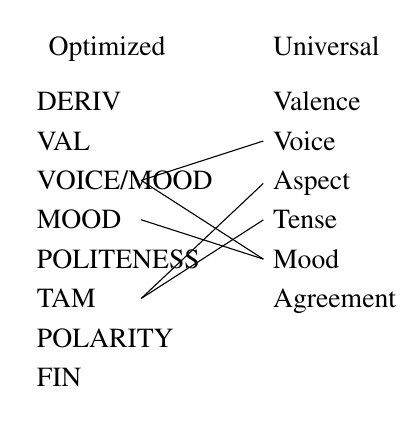
\begin{tikzpicture}[%
% common options for blocks:
block/.style = {draw, fill=blue!30, align=center, anchor=west,
            minimum height=0.65cm, inner sep=0},
% common options for the circles:
ball/.style = {circle, draw, align=center, anchor=north, inner sep=0}]
\node[rectangle,text width=1.2cm,anchor=base] (A0) at (4,-0.3) {Universal};
\node[rectangle,text width=0.9cm,anchor=base] (B0) at (1,-0.3) {Optimized};
\node[rectangle,text width=1.2cm,anchor=base] (A1) at (4,-1.0) {Valence};
\node[rectangle,text width=1.2cm,anchor=base] (A2) at (4,-1.5) {Voice};
\node[rectangle,text width=1.2cm,anchor=base] (A3) at (4,-2.0) {Aspect};
\node[rectangle,text width=1.2cm,anchor=base] (A4) at (4,-2.5) {Tense};
\node[rectangle,text width=1.2cm,anchor=base] (A5) at (4,-3.0) {Mood};
\node[rectangle,text width=1.2cm,anchor=base] (A6) at (4,-3.5) {Agreement};
\node[rectangle,text width=1.2cm,anchor=base] (B1) at (1,-1.0) {DERIV};
\node[rectangle,text width=1.2cm,anchor=base] (B2) at (1,-1.5) {VAL};
\node[rectangle,text width=1.2cm,anchor=base] (B3) at (1,-2.0) {VOICE/MOOD};
\node[rectangle,text width=1.2cm,anchor=base] (B4) at (1,-2.5) {MOOD};
\node[rectangle,text width=1.2cm,anchor=base] (B5) at (1,-3.0) {POLITENESS};
\node[rectangle,text width=1.2cm,anchor=base] (B6) at (1,-3.5) {TAM};
\node[rectangle,text width=1.2cm,anchor=base] (B7) at (1,-4.0) {POLARITY};
\node[rectangle,text width=1.2cm,anchor=base] (B8) at (1,-4.5) {FIN};
\draw[-] (A2.west) to (B3.east);
\draw[-] (A5.west) to (B3.east);
\draw[-] (A5.west) to (B4.east);
\draw[-] (A3.west) to (B6.east);
\draw[-] (A4.west) to (B6.east);
\end{tikzpicture}

    \end{minipage}
        &
    \begin{minipage}{.3\textwidth}
    \begin{tikzpicture}[%
% common options for blocks:
block/.style = {draw, fill=blue!30, align=center, anchor=west,
            minimum height=0.65cm, inner sep=0},
% common options for the circles:
ball/.style = {circle, draw, align=center, anchor=north, inner sep=0}]
\node[rectangle,text width=1.2cm,anchor=base] (A0) at (4,-0.3) {Universal};
\node[rectangle,text width=0.9cm,anchor=base] (B0) at (1,-0.3) {Optimized};
\node[rectangle,text width=1.2cm,anchor=base] (A1) at (4,-1.0) {Valence};
\node[rectangle,text width=1.2cm,anchor=base] (A2) at (4,-1.5) {Voice};
\node[rectangle,text width=1.2cm,anchor=base] (A3) at (4,-2.0) {Aspect};
\node[rectangle,text width=1.2cm,anchor=base] (A4) at (4,-2.5) {Tense};
\node[rectangle,text width=1.2cm,anchor=base] (A5) at (4,-3.0) {Mood};
\node[rectangle,text width=1.2cm,anchor=base] (A6) at (4,-3.5) {Agreement};
\node[rectangle,text width=1.2cm,anchor=base] (B1) at (1,-1.0) {Other_6};
\node[rectangle,text width=1.2cm,anchor=base] (B2) at (1,-1.5) {Other_2a};
\node[rectangle,text width=1.2cm,anchor=base] (B3) at (1,-2.0) {Infinitive};
\node[rectangle,text width=1.2cm,anchor=base] (B4) at (1,-2.5) {Other_ij};
\node[rectangle,text width=1.2cm,anchor=base] (B5) at (1,-3.0) {Other_wo};
\node[rectangle,text width=1.2cm,anchor=base] (B6) at (1,-3.5) {Other_di};
\node[rectangle,text width=1.2cm,anchor=base] (B7) at (1,-4.0) {Other_copula};
\node[rectangle,text width=1.2cm,anchor=base] (B8) at (1,-4.5) {Other_1s};
\node[rectangle,text width=1.2cm,anchor=base] (B9) at (1,-5.0) {Other_lo};
\node[rectangle,text width=1.2cm,anchor=base] (B10) at (1,-5.5) {Subject};
\node[rectangle,text width=1.2cm,anchor=base] (B11) at (1,-6.0) {Other_f^};
\node[rectangle,text width=1.2cm,anchor=base] (B12) at (1,-6.5) {Other_2};
\node[rectangle,text width=1.2cm,anchor=base] (B13) at (1,-7.0) {Tense/aspect};
\node[rectangle,text width=1.2cm,anchor=base] (B14) at (1,-7.5) {Int/Rel};
\node[rectangle,text width=1.2cm,anchor=base] (B15) at (1,-8.0) {Other_av};
\node[rectangle,text width=1.2cm,anchor=base] (B16) at (1,-8.5) {Negation};
\node[rectangle,text width=1.2cm,anchor=base] (B17) at (1,-9.0) {Other_9};
\node[rectangle,text width=1.2cm,anchor=base] (B18) at (1,-9.5) {Other_3};
\node[rectangle,text width=1.2cm,anchor=base] (B19) at (1,-10.0) {Other_17};
\node[rectangle,text width=1.2cm,anchor=base] (B20) at (1,-10.5) {Other_10};
\node[rectangle,text width=1.2cm,anchor=base] (B21) at (1,-11.0) {Other_7};
\node[rectangle,text width=1.2cm,anchor=base] (B22) at (1,-11.5) {Other_pr};
\node[rectangle,text width=1.2cm,anchor=base] (B23) at (1,-12.0) {Object/reflexive};
\draw[-] (A6.west) to (B10.east);
\draw[-] (A3.west) to (B13.east);
\draw[-] (A4.west) to (B13.east);
\draw[-] (A1.west) to (B23.east);
\end{tikzpicture}

    \end{minipage}
    \\
    \textsc{Sesotho Suffixes} \\
        \begin{minipage}{.3\textwidth}
    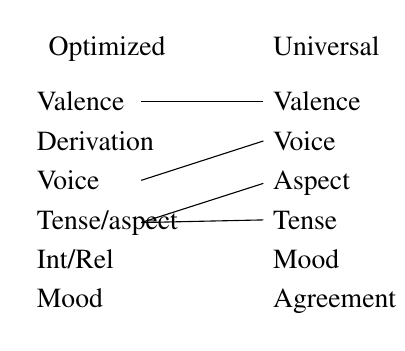
\begin{tikzpicture}[%
% common options for blocks:
block/.style = {draw, fill=blue!30, align=center, anchor=west,
            minimum height=0.65cm, inner sep=0},
% common options for the circles:
ball/.style = {circle, draw, align=center, anchor=north, inner sep=0}]
\node[rectangle,text width=1.2cm,anchor=base] (A0) at (4,-0.3) {Universal};
\node[rectangle,text width=0.9cm,anchor=base] (B0) at (1,-0.3) {Optimized};
\node[rectangle,text width=1.2cm,anchor=base] (A1) at (4,-1.0) {Valence};
\node[rectangle,text width=1.2cm,anchor=base] (A2) at (4,-1.5) {Voice};
\node[rectangle,text width=1.2cm,anchor=base] (A3) at (4,-2.0) {Aspect};
\node[rectangle,text width=1.2cm,anchor=base] (A4) at (4,-2.5) {Tense};
\node[rectangle,text width=1.2cm,anchor=base] (A5) at (4,-3.0) {Mood};
\node[rectangle,text width=1.2cm,anchor=base] (A6) at (4,-3.5) {Agreement};
\node[rectangle,text width=1.2cm,anchor=base] (B1) at (1,-1.0) {Valence};
\node[rectangle,text width=1.2cm,anchor=base] (B2) at (1,-1.5) {Derivation};
\node[rectangle,text width=1.2cm,anchor=base] (B3) at (1,-2.0) {Voice};
\node[rectangle,text width=1.2cm,anchor=base] (B4) at (1,-2.5) {Tense/aspect};
\node[rectangle,text width=1.2cm,anchor=base] (B5) at (1,-3.0) {Int/Rel};
\node[rectangle,text width=1.2cm,anchor=base] (B6) at (1,-3.5) {Mood};
\draw[-] (A1.west) to (B1.east);
\draw[-] (A2.west) to (B3.east);
\draw[-] (A3.west) to (B4.east);
\draw[-] (A4.west) to (B4.east);
\end{tikzpicture}

    \end{minipage}
\end{tabular}
    \caption{Comparing optimized orders of verb affixes with the universal order described by \citep{bybee-morphology-1985}. \mhahn{It might be possible to remove this figure and instead indicate the match by introducing color coding to Figure 8, so it would become visually obvious there. What do you think?}}
    \label{fig:optimized_and_universal_orders}
\end{figure}



\begin{table}[]
    \centering
    \begin{tabular}{l|l|l|ll|ll|llllll}
%    &     &    \multicolumn{2}{c|}{Pairs} & \multicolumn{2}{c|}{Full} & \multicolumn{2}{c}{Full (Types)} \\
%      &   &     Optim. & Baseline & Quantile. & 95\% CI  & Optim. & Baseline \\ \hline
%     &   &     Optim. & Baseline & Quantile  \\ \hline
     &   &     Optim. & \multicolumn{2}{|c}{Baseline (Random)} & \multicolumn{2}{|c|}{Baseline (Universals)}  \\ 
     &  &            & Accuracy & Quantile & Accuracy & Quantile \\
     \hline
     \multirow{3}{*}{Nouns} & Finnish & 1.0 (0.0) & 0.52 (0.32) & 1.0  [0.95, 1.0]  \\
 & Turkish & 1.0 (0.0) & 0.54 (0.36) & 1.0  [0.95, 1.0]  \\
 & Hungarian & 1.0 (0.0) & 0.47 (0.37) & 1.0  [0.95, 1.0]  \\
\hline
\multirow{7}{*}{Verbs} & Finnish & 0.4 (0.3) & 0.57 (0.38) & 0.43  [0.34, 0.52]  \\
 & Hungarian & 0.95 (0.09) & 0.52 (0.4) & 0.81  [0.72, 0.88]  \\
 & Turkish & 0.96 (0.09) & 0.52 (0.14) & 1.0  [0.96, 1.0]  \\
 & Korean & 0.97 (0.1) & 0.55 (0.24) & 1.0  [0.95, 1.0]  \\
 & Japanese & 0.95 (0.0) & 0.48 (0.24) & 1.0  [0.85, 1.0]  \\
 & Sesotho (P) & 0.98 (0.0) & 0.56 (0.48) & 0.77  [0.65, 0.86]  \\
 & Sesotho (S) & 0.62 (0.0) & 0.43 (0.23) & 0.82  [0.72, 0.9]  \\

    \end{tabular}
    \caption{Accuracies in predicting morpheme ordering. `Optim.' indicates grammars optimized for AUC, `'Baseline' indicates randomly constructed weights.
    In each cell, we provide the mean and the standard deviation over orderings.
    We also show the fraction of baseline orderings with lower accuracy than the optimized order, with a 95\% binomial confidence interval.
    \mhahn{could think about making this a set of small violin plots for each language, instead of providing numerical hard-to-think-about quantile information}
    }
    \label{tab:optimized_acc}
\end{table}















\subsection{Relation to previous accounts}



\paragraph{Relation to Previous Theories} here explain link to bybee

We suggest that mutual information provides an operational formalization of semantic relevance. \becky{Should this be explained earlier in the paper?}
For instance, we expect that passive markers have a high mutual information with the verb stem, since only certain verbs (typically a subclass of the transitive verbs) can form a passive.
The idea that mutual information is an operationalization of semantic closeness has also been suggested in other places; for instance, \citep{culbertson2020from} link mutual information to conceptual closeness as a driving factor of noun phrase modification.

\mhahn{I'm pondering to what extent it would be helpful to expound on the connection between the tradeoff and locality, to make the link to Bybee.} \jd{i think it would be very helpful. currently the connection to bybee feels a little off the cuff and unmotivated. it would be worth being more explicit about bybee's notion of relevance, and why we think MI is a good formalization of it.}




%\subsubsection{Semantic Scope; Syntactic Structure; Historical Development}
%Morpheme ordering has been described from the perspective 
%Besides the explanation of broad typological tendencies, which we are interested in here, the linguistic literature has also debated at which level of linguistic representation morpheme ordering should be described, proposing accounts located at different levels such as the syntax-phonology interface \citep{baker1985the} and an autonomous layer of morphological description \citep{hyman2003suffix}.
%TODO also template vs scope vs...
%We do not see the memory--surprisal tradeoff as competing with or contradicting these studies.
%Rather, it specifies tendencies for ordering that could be implemented at different levels of linguistic description.

%\paragraph{Revelance and Proximity}


%A related family of explanations holds that those affixes are closest to the root that are most relevant to the root.
%Our optimized orders of Turkish and Hungarian \becky{Are there other languages?} perfectly match Bybee's proposed universal verbal inflection order (Figure REF).
%This suggests that high mutual information generally correlates with semantic relevance. 


In this section, we relate our results to existing explanatory accounts of morpheme ordering.
In a review of research on morpheme ordering, \citet{manova2010modeling} % https://homepage.univie.ac.at/stela.manova/modeling%20affix%20order.pdf
categorize approaches to morpheme ordering into three classes (similarly \citet{rice2000morpheme, rice2011principles}): orderings that are motivated by properties of syntax, semantics or phonology; orderings that are motivated by human language processing responding to statistical properties of language; and orderings that are arbitrarily stipulated.
%Our approach falls into the second class, explaining morpheme ordering based on minimization of human processing effort.
In this section, we describe how our account relates to other accounts across these three \becky{four?} clusters, and show how the memory-surprisal tradeoff has tight connections with notions proposed across seemingly very different accounts.

%\mhahn{One can debate whether this trichotony is right -- e.g. Bybee's approach could be thought of as cognitive. What the second class 


%- citing \cite{rice2000morpheme}; Manova and Aronoff 2010; Saarinen and Hay 2014
%Rice states three types of explanations/phenomena:
%- extra-grammatical: frequency, productivity, parsability


\subsubsection{Relations to Syntactic Theories}

A family of theories hold that morpheme ordering is motivated by constraints placed on morphology through the interaction with other aspects of grammar.
The approaches most relevant for our results are approaches in terms of the relation of morphology to syntax~\citep{baker1985the} and semantics~\citep{bybee-morphology-1985,rice2000morpheme}.

%- grammatuical principle (syntactic, semantic, phonological). famous examples Mirror Principle and Bybee's relevance Principle; Scope (Rice)


%Mirror princuiple built into Distributed Morphology (Harley and Noyer 1998)

%\mhahn{report the following somewhere}
%We measured the mutual information between roots and features using the other Universal Dependencies corpora for which these features were available.
%First, for nouns, we compared the mutual information between the lemma and case and number, using a mixed-effects model with random effects for languages and language families.
%Across 34 languages, mutual information tended to be higher for number than for case ($\beta=0.04$, $SE=0.015$, $t=2.58$, 30 languages).
%For verbs, we compared mutual information between the root and voice, TAM, and subject agreement features.
%Mutual information was higher for TAM than for agreement ($\beta=0.1$, $SE=0.04$, $t=2.29$, 37 languages), however, there was no significant difference between TAM and voice ($\beta=0.08$, $SE=0.058$, $t=1.39$, 30 languages).


%TODO think about where to explain this As mentioned in section \becky{cite S2}, Bybee proposes a concept of \textit{semantic relevance}, which is the degree to which one morpheme affects the semantic content of the other \becky{cite bybee}. She hypothesizes that morphemes that are more highly relevant to each other should be closer to each other, and therefore proposes a universal ordering of verbal inflectional morphemes. For example, attaching a causative marker to a root meaning "to die" produces a verb form meaning "to kill." Since the causative greatly changes the semantic content of the original root, the causative is highly relevant to the root. 
%\becky{Format Korean example of juk-da ``to die" and juk-i-da ``to kill"}
%Bybee did not provide a way to computationally measure semantic relevance. 


%Other explanations suggest that morphemes are ordered based on (TODO CITE).
%The most straightforwardly related account is that of Bybee (1985) Semantic relevance
%CARP template in Bantu
%Explanations for the orders

%talk about Relevance and Mutual Information
%\paragraph{Morphemes as Fossilized Words}\

It has long been observed that the order of morphemes often parallels the order of independent words of corresponding meanings \citep{givon1971historical,venneman1973explanation,baker1985the}.
One explanation for this is that the order of morphemes reflects the order of formerly independent elements that have been fossilized into bound morphemes, which can often be verified in languages where historical data is available \citep{givon1971historical,venneman1973explanation}.
% interesting: Evans, Nicholas (1995). Multiple case in Kayardild: Anti-iconic suffix ordering and the diachronic filter. In Plank (ed.) 1995, 396-430. 
% Moravcsik, Edith A. (1995). Summing up Suffixaufnahme. In Plank (ed.) 1995, 451-484.  HEREL : 478, G24
% Cited by https://typo.uni-konstanz.de/rara/universals-archive/41/
On the other hand, \citet{bybee-morphology-1985} points out that there are historically documented cases where morpheme ordering has been restructured in ways that do not reflect former independent words, but respect the universal tendencies proposed by her \becky{``that she proposed" instead of ``proposed by her" ?} (see also \citet{mithun2000the, haspelmath1993the, mithun1995affixation}; \citet[Section 15]{rice2000morpheme}).
A correspondence between the order of words and morphemes has also been postulated on a purely synchronic basis as a constraint on possible human languages.
\cite{baker1985the} proposed the Mirror Principle, which -- informally -- states that the order of elements (morphemes) in morphology reflects the order of elements (words) in syntax.
A large body of work in theoretical syntax describes word and morpheme order using the same processes and principles \citep{halle1993distributed}.
As a theory of order at multiple levels, the Efficient Tradeoff Hypothesis is compatible with these different historical paths and predicts these ordering patterns independently of the historical path leading to the morphemes found in a given language.



%As the memory-surprisal tradeoff is optimized by word order, this is compatible with our results:
%To the extent that morpheme order does reflect fossilized word order, morpheme order should continue to reflect optimization for the tradeoff.


%To the extent that similar statistical patterns of usage hold for corresponding words and morphemes, this again is compatible with the Efficient Tradeoff Hypothesis.

%\mhahn{TODO regarding scope: \citep{baker1988incorporation,foley1984functional,chierchia1990meaning,valin1992a}}


%This can be related to the scope-based explanation to the extent that syntactic structure and word order reflect scope.
% INTERESTING reference: http://www.jzeller.de/pdf/CARP.pdf

%\paragraph{Semantic Scope}


%Description in terms of scope faces limitations when order is different from semantic scope.
%\cite{Hyman2003}
%Hyman  (2003:  249) proposed the CARP template to describe suffix order in Bantu languages (such as Sesotho), a templatic order for valence and voice morphemes that can be different from scope order.
%In \cite{Hyman2003}'s model, order is determined based on both the CARP template and a preference for ismorphism with semantic scope.
%


%The principle of semantic scope is explained in detail and illustrated with copiousexamples in \cite{caballero2010scope}. \cite{narrog2010the} and most of the papers included in thenext issue provide analyses based on semantic scope, Aronoff and Xu (next issue),Korotkova and Lander (next issue), and Nordlinger (next issue).




Other prominent accounts are in terms of a correspondence between morpheme ordering and semantics~\citep{bybee-morphology-1985,rice2000morpheme}.
\citet{bybee-morphology-1985} argues that semantic relevance determines ordering.
For example, morphemes changing a verb's argument structure, such as passives and causatives, have a particularly strong relation to the verb's semantics, as they fundamentally alter the nature of the event described, whereas tense or agreement markers are much less tightly linked the the verb's meaning.
We suggest that mutual information provides an operational formalization of semantic relevance. \becky{Should this be explained earlier in the paper?}
For instance, we expect that passive markers have a high mutual information with the verb stem, since only certain verbs (typically a subclass of the transitive verbs) can form a passive.
The idea that mutual information is an operationalization of semantic closeness has also been suggested in other places; for instance, \citep{culbertson2020from} link mutual information to conceptual closeness as a driving factor of noun phrase modification.

A second prominent semantic account is in terms of semantic scope \citep{rice2000morpheme}.
This is the idea that morphemes are ordered in the order in which their meanings combine \citep[e.g.,][]{rice2000morpheme, caballero2010scope,  narrog2010the, korotkova2010deriving}.
The relative ordering of valence and voice is a good example for the scope-based explanation.
Valence affixes change the number of arguments, and passive (voice) promotes one argument to the subject position.
This can affect an argument introduced by a voice marker.
The following example from Turkish illustrates this (\cite{schaaik2020turkish}, section 30.8.2):


\begin{tabular}{ccccccc}
don-dur-ul & freeze-caus-pass & be frozen \\
don-dur & freeze-caus & to freeze (something) \\
don & freeze& to freeze \\
\end{tabular}

Turkish has suffixes both for causative and passive.
When adding both suffixes simultaneously, the causative marker appears closer to the root.
This corresponds to the order in which the meanings of these suffixes combine with the meaning of the root:
Causative adds an argument indicating who makes an object freeze, and passive then removes that argument, yielding a verb describing something that is being frozen by someone.

A priori, semantic scope is different from mutual information.
However, there are arguments that scope relations correlate with mutual information.
\citet{culbertson2020from} made a related argument for the order of nominal modifiers as in ``the four green books'', where mutual information predicts the order of attachment of modifiers to the noun.
%Furthermore, if the semantic propositions that speakers communicate are modeled using a probabilistic language-of-thought grammar such as mutual information will also correlate with scope ordering (see SI Appendix Section S4 for a simulation study).




\subsubsection{Motivations in Terms of Human Language Processing}

A prominent cognitively-motivated theory of morpheme ordering is the theory of Complexity-Based Ordering \citep{hay2002speech,plag2002the,hay2004what,hay2005shifting,plag2009suffix}.
This theory holds that affixes are closer to the root when they are less ``separable'', where separability indicates the productivity of an affix and the likelihood that affixes are processed separately with the base in human lexical access  \citep{baayen1993on}.
%In particular, affixes are less ``separable'' when they are processed holistically together with the base in human lexical access \citep{baayen1993on}. %, such as in the dual processing race model of morphological access, which asserts that morphological forms can be processed either separately in terms of its components or as a whole \citep{baayen1993on}.
%Forms are more separable if they are less likely to be processed together with the root (Baayen \& Schreuder 1999, Baayen \& Moscoso del Prado Mart ́ın 2005).
%also mention \cite{manova2010suffix}
%\cite{plag2009suffix} %http://www.sfs.uni-tuebingen.de/~hbaayen/publications/plagBaayenLanguage2009.pdf
A statistical operationalization of separability is in terms of relative frequencies:
affixes are more likely to be processed together with the root when the composite form has a higher frequency compared to the base form \citep{hay2001lexical}. % , lee2011ordering
This has an interesting relation to mutual information: 
If the compound form is very frequent, in relation to the baseline frequencies of the base and the affix, then there is high (pointwise) mutual information between them.
\mhahn{Make clear that this theory hasn't been applied to the kinds of affix orderin generalizations that we look at in this paper.}

Most closely related to our proposal, \citet{inkelas2016affix} proposed that morphemes are ordered together when they are informative about each other.
They considered a notion of informativity introduced by \citet{priva2017informativity}, which is different from but related to the mutual information between adjacent morphemes $I_1$ (see SI Appendix Section S3 for details).
%Formally (drawing on the notion of informativity defined by \citet{priva2017informativity}), they considered the informativity between a suffix $S_i$ and the preceding $S_{i-1}$ as 
%\begin{equation}
%    \sum_{S_{i-1}, S_{i}} \frac{P(S_{i-1} , S_i)}{P(S_i)} \log P(S_i | S_{i-1})
%\end{equation}
They tested this idea in a pilot study of Turkish, finding that high-informativity suffixes are closer to the root.
%This notion of informativity is similar to $I_1$, only differing in whether the $P(S_i)$ term occurs inside the logarithm:
%\begin{equation}
%   I_1 = \sum_{S_{i-1}, S_{i}} P(S_{i-1} , S_i) \log \frac{P(S_i | S_{i-1})}{P(S_i)}
%\end{equation}


%Inkelas: informativity: they propose that bigram surprisal is minimized (not their terminology), test this in a pilot study of Turkish, with partially confirming results \citep{inkelas2015informativity}
%Alternatively, the lower thefrequency of the derived word in relation to the base word, the more important the role ofthe constituents become
%Hay and Plag (2004) show that ordering correlates with relative frequency and productivity
%Hay (in press) distinguishes between derived forms which are more frequent than the bases they contain (e.g.illegible is more frequent than legible), and derived forms whic hare less frequent than their bases (e.g.illiberal is less frequent than liberal).
% argues that whether an affix is processed together with the root is determined in part by the relative frequency
%\begin{equation}
%    \frac{P(base+affix)}{P(base)}
%\end{equation}
%\begin{equation}
%    \log \frac{P(base, affix)}{P(base)} = \log P(affix|base)
%\end{equation}
%\begin{equation}
%    pmi(base, affix) = \log \frac{p(affix|base)}{p(base)}
%\end{equation}
%Hay and Baayen (2002).
%Hay and Plag (2004): parsing ratio and productivity measured by Hay and Baayen (2002).
%Complexity-based Ordering, the position of a given suffix inthe hierarchy reflects the degree to which that suffix is processed independently of its base.

%\citet{hay2004what} propose a model of complexity-based ordering based on processing considerations, called complexity-based ordering, arguing that affixes are further away from the root when they can be separated more easily in processing, testing this theory using 15 English affixes.


%from Inkelas



\subsubsection{Arbitrary Orderings}

There are also studies suggesting language-specific and essentially arbitrary properties of morpheme ordering.
A classical approach to describing morpheme ordering is in terms of levels, where morphemes from a higher level occur before morphemes from a lower level \citep{siegel1979topics}, and in terms of templates that describe the ordering of morphemes \citep{simpson1986pronominal,spencer1991morphological,stump1992on,inkelas1993nimboran,hyman2003suffix,nordlinger2010verbal}.
Ordering based on language-specific templates has been proposed specifically in cases where observed morpheme ordering is in conflict with semantic scope, as in Bantu languages \citep{hyman2003suffix}.
\citet{fabb1988english} prominently describes English affix ordering in terms of the selectional restrictions that individual affixes place on which other affixes they can attach to.
While this approach does not make statements as to which affixes would go closer to the base in a given language, it does suggest that morpheme ordering is described based on the pairwise interactions between adjacent morphemes.
In a similar vein, \citet{ryan2010variable} propose a model based on weighted bigram constraints in Tagalog, for the (rather uncommon) case of flexible morpheme ordering.
Ordering constraints operating on adjacent pairs of morphemes might provide relatively efficient memory-surprisal tradeoffs because the appearance of a morpheme is constrained only by its immediately adjacent morphemes.




%Tension between Scope and templatic: \citep{hyman2003suffix}; \cite{aronoff2010introduction}; \cite{spencer2003putting}
%- arbitrary language-specific tenplatic (Fabb 1988 English affix ordering; position class templates, Simpson and Withgott 1986) (also finite-state automata Hankamer 1986; Karttunen 2003) 

%re scope also \cite{alsina1999where}

%\cite{manova2010modeling} % https://homepage.univie.ac.at/stela.manova/modeling%20affix%20order.pdf
%also provide a ctagoeirzation into grammatical, psycholinguistic, unmotivated (among others)





%\cite{aronoff2010a} % Within this model, phonological form is spelled out by means of individual-language-particular realization constraints that associate abstract morphosyntactic feature values with phonological forms and that are ordered among more general constraints governing factors like scope and feature splitting. The data used to exemplify the application of our theory to affix order are drawn from Haspelmath’s (A grammar of Lezgian, Mouton de Gruyter, Berlin, 1993) grammar of Lezgian, a language of the Northeast Caucasian family spoken largely in Dagestan (Russia) and Azerbaijan.



%\paragraph{Templates}
%CARP template
%\cite{muysken1981quechua}
%\cite{mccarthy2008generalized} phonology
%\cite{hyman2003suffix}
%\cite{kanu2009suffix} morphotactics, not semantic scope





%\subsubsection{Semantic Scope; Syntactic Structure; Historical Development}
%Morpheme ordering has been described from the perspective 
%Besides the explanation of broad typological tendencies, which we are interested in here, the linguistic literature has also debated at which level of linguistic representation morpheme ordering should be described, proposing accounts located at different levels such as the syntax-phonology interface \citep{baker1985the} and an autonomous layer of morphological description \citep{hyman2003suffix}.
%TODO also template vs scope vs...
%We do not see the memory--surprisal tradeoff as competing with or contradicting these studies.
%Rather, it specifies tendencies for ordering that could be implemented at different levels of linguistic description.

%\paragraph{Revelance and Proximity}


%A related family of explanations holds that those affixes are closest to the root that are most relevant to the root.
%Our optimized orders of Turkish and Hungarian \becky{Are there other languages?} perfectly match Bybee's proposed universal verbal inflection order (Figure REF).
%This suggests that high mutual information generally correlates with semantic relevance. 